%%%%%%%%%%%%%%%%%%%%%%%%%%%%%%%%%%%%%%%%
%% Formato para revista ASOiMAT basado en la clase
%% aleph-revista, versión 1.0 (13/06/2021)
%%%%%%%%%%%%%%%%%%%%%%%%%%%%%%%%%%%%%%%%
\documentclass{aleph-revista}

%%%%%%%%%%%%%%%%%%%%%%%%%%%%%%%%%%%%%%%%
%% Declaración de paquetes adicionales
%%%%%%%%%%%%%%%%%%%%%%%%%%%%%%%%%%%%%%%%
%% Aquí incluya los paquetes necesarios para su documento. 
%% No incluya paquetes que no sean necesarios. 
%% Estos son ejemplos de paquetes que le pueden ser de utilidad.
%% Si no los va a utilizar, eliminarlos.
\usepackage{tikz}           % Para generar gráficos 
\usepackage{aleph-comandos} % Comandos para facilitar escritura matemática
\usepackage{multicol}       % Para utilizar multicolumnas
\addbibresource{Bibliografia.bib}         % Archivo de bibliografía

%%%%%%%%%%%%%%%%%%%%%%%%%%%%%%%%%%%%%%%%
%% Declaración de comandos adicionales
%%%%%%%%%%%%%%%%%%%%%%%%%%%%%%%%%%%%%%%%
%% Aquí incluya los definiciones de comandos necesarios para 
%% su documento.
%%%%%%%%%%%%%%%%%%%%%%%%%%%%%%%%%%%%%%%%
%% Datos del la publicación
%%%%%%%%%%%%%%%%%%%%%%%%%%%%%%%%%%%%%%%%
\volumen{1}
\numero{1}
\fechapubli{2021}
\periodouno{Marzo}
\periododos{Junio}
%%%%%%%%%%%%%%%%%%%%%%%%%%%%%%%%%%%%%%%%
%% Datos del artículo
%%%%%%%%%%%%%%%%%%%%%%%%%%%%%%%%%%%%%%%%
\titulo{ANÁLISIS DE VIBRACIONES LIBRES EN ROBOT KR 1000 TITAN}

\tituloingles{FREE VIBRATIONS ANALYSIS IN ROBOT KR 1000 TITAN}

\autor{%
    Bustillo, Carlos\textsuperscript{1 \faEnvelopeO}; 
    Linares, Ramiro\textsuperscript{1\faEnvelopeO}; 
    Pérez, Rodrigo\textsuperscript{1\faEnvelopeO}
}

\institucion{
\textsuperscript{1}%
    Facultad de Ingeniería, Universidad Nacional de Cuyo, Mendoza, Argentina
}

\correo{cabustillo13@hotmail.com;   rodrigoperez2110@gmail.com; ramylinares@gmail.com}

\fecha{27 de junio de 2021}

\resumen{
   El KR 1000 TITAN es un robot industrial de 6 GDL diseñado para trabajar con cargas pesadas a elevada rapidez y precisión, hasta una distancia de 6,5 m. Se lo utiliza para manipular bloques de motor, piedras, piezas de vidrio, vigas de acero, piezas navales y aeronáuticas, bloques de mármol o prefabricados de hormigón, entre otros muchos. Nuestro análisis onsiste en realizar un estudio vibratorio, para poder asegurar que las oscilaciones producidas no sean demasiado grandes como para interferir en la operación que lleve a cabo el robot en dicha posición. Al agarrar un objeto, se le suma su masa a la del sistema, y se determinará cómo esto influye en su vibración libre.
 
}
\palabrasc{Robot KUKA, Vibraciones Libres, Modos de vibración.}

\abstract{
    The KR 1000 TITAN is a 6 DOF industrial robot designed to work with heavy loads at high speed and precision, up to a distance of 6.5 m. It is used to manipulate engine blocks, stones, glass pieces, steel beams, naval and aeronautical pieces, marble blocks or precast concrete, among many others. Our analysis consists in carrying out a vibratory study, in order to ensure that the oscillations produced are not too large to interfere with the operation carried out by the robot in that position. When grasping an object, its mass is added to that of the system, and it will be determined how this influences its free vibration.
}
\keywords{KUKA robot, Free Vibrations, Vibration modes.}

\begin{document}
%%%%%%%%%%%%%%%%%%%%%%%%%%%%%%%%%%%%%%%%
%% Encabezado
%%%%%%%%%%%%%%%%%%%%%%%%%%%%%%%%%%%%%%%%
\membrete

%%%%%%%%%%%%%%%%%%%%%%%%%%%%%%%%%%%%%%%%
\section{Introducción}
%%%%%%%%%%%%%%%%%%%%%%%%%%%%%%%%%%%%%%%%
El KR 1000 TITAN, es un robot industrial de 6 grados de libertad gdl  con 6 respectivos servomotores, diseñado para trabajar con cargas pesadas de más de 1000 kg, a elevada rapidez y precisión, y hasta una distancia de 6,5 m. Se utiliza para manipular bloques de motor, piedras, piezas de vidrio, vigas de acero, piezas navales y aeronáuticas, bloques de mármol o prefabricados de hormigón, entre otros muchos.

Se realizará un estudio vibratorio de dicho robot kuka, para corroborar su correcto funcionamiento ante vibraciones libres. Lo cual es de gran interés sobre todo por el enorme peso y gran velocidad que maneja el robot, para verificar si su precisión se mantiene aceptable.

En el movimiento programado, con el cual el robot realiza una operación genérica determinada, se captura un instante en el cual detiene su movimiento, trabando los motores. En dicha posición se estudiará el sistema en vibraciones libres, en forma similar a como si se tratara de una estructura fija. En donde, las vibraciones libres se manifestarán por la energía cinética, de la inercia del robot y de la masa que manipula, en dicho instante de tiempo. Y se representan mediante las condiciones iniciales de velocidad del sistema dinámico. Por otro lado, las condiciones iniciales de posición se las considera nulas, lo que significa que el robot se encuentra en la posición exacta en la que los motores se encuentran trabados, y sin vibrar.
Debido a la rígida estructura del robot, se considera que los parámetros de rigidez y amortiguamiento solamente se encuentran dados por los propios motores, y no por los materiales de los eslabones en sí. Esto es debido a que, en comparación, los efectos de los materiales sobre la respuesta de las vibraciones, son despreciables. Es decir, para el estudio solo se considerarán las rigideces y amortiguamientos de los servomotores.

\begin{figure}[H]
    \centering
    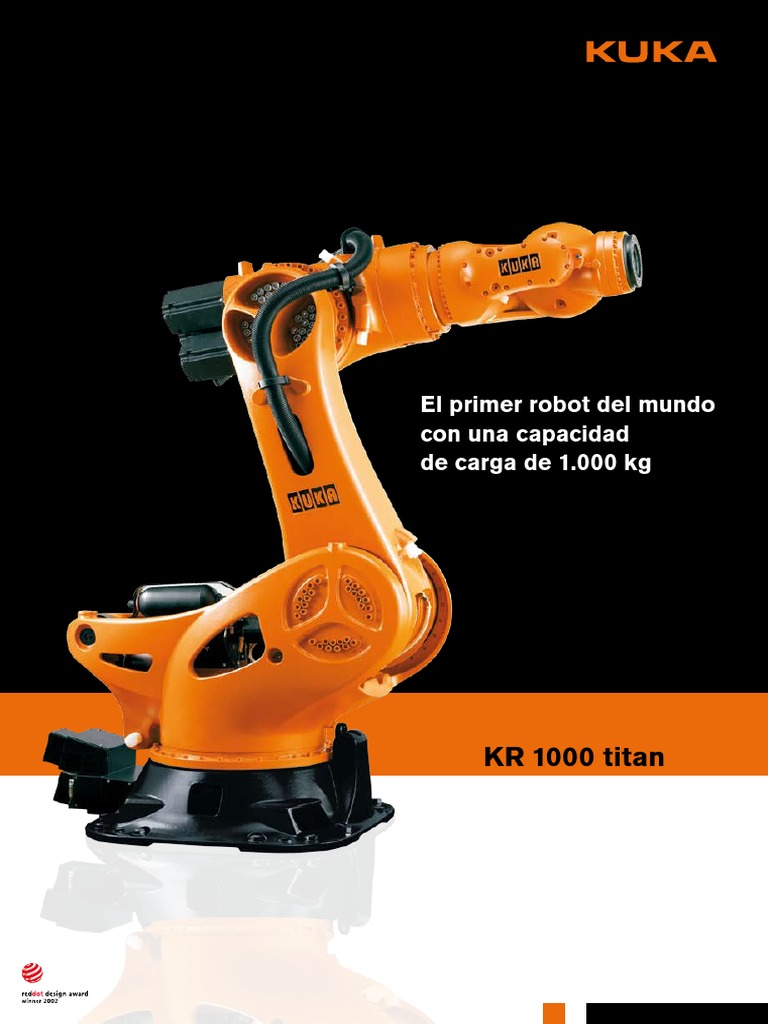
\includegraphics[width=0.60\textwidth]{Imagenes/modelo_2.jpg}
    \caption{Robot KUKA KR 1000 TITAN.}
    \label{fig:etiqueta de la figura}
\end{figure}

El objetivo consiste en realizar un estudio vibratorio, para poder asegurar que las oscilaciones producidas no sean demasiado grandes como para interferir en la operación que lleve a cabo el robot.
Desarrollando un modelo físico y matemático del sistema dinámico real, obteniendo su respuesta, y modificando los parámetros que pueden variar de una aplicación a otra, para obtener conclusiones acerca de cómo esto influye, y qué tan bueno es su diseño respecto a las vibraciones.En particular, modificando los parámetros de la masa de la carga que manipula, y las velocidades iniciales del sistema.

\begin{figure}[H]
    \centering
    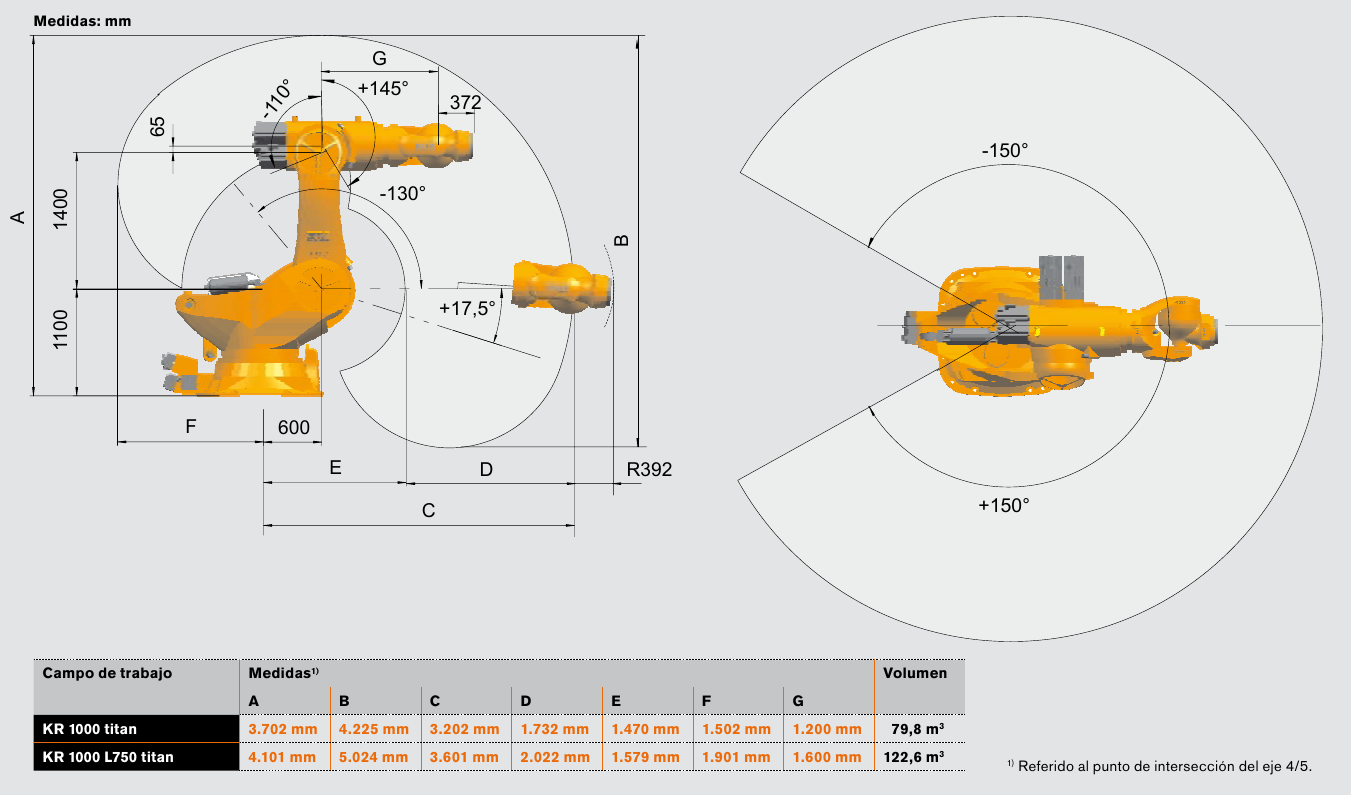
\includegraphics[width=0.60\textwidth]{Imagenes/area_trabajo.png}
    \caption{Área de trabajo.}
    \label{fig:etiqueta de la figura}
\end{figure}

%%%%%%%%%%%%%%%%%%%%%%%%%%%%%%%%%%%%%%%%
\section{Modelo}
%%%%%%%%%%%%%%%%%%%%%%%%%%%%%%%%%%%%%%%%

El modelado del problema es uno de los ejes principales considerados en este proyecto.

\begin{figure}[H]
    \centering
    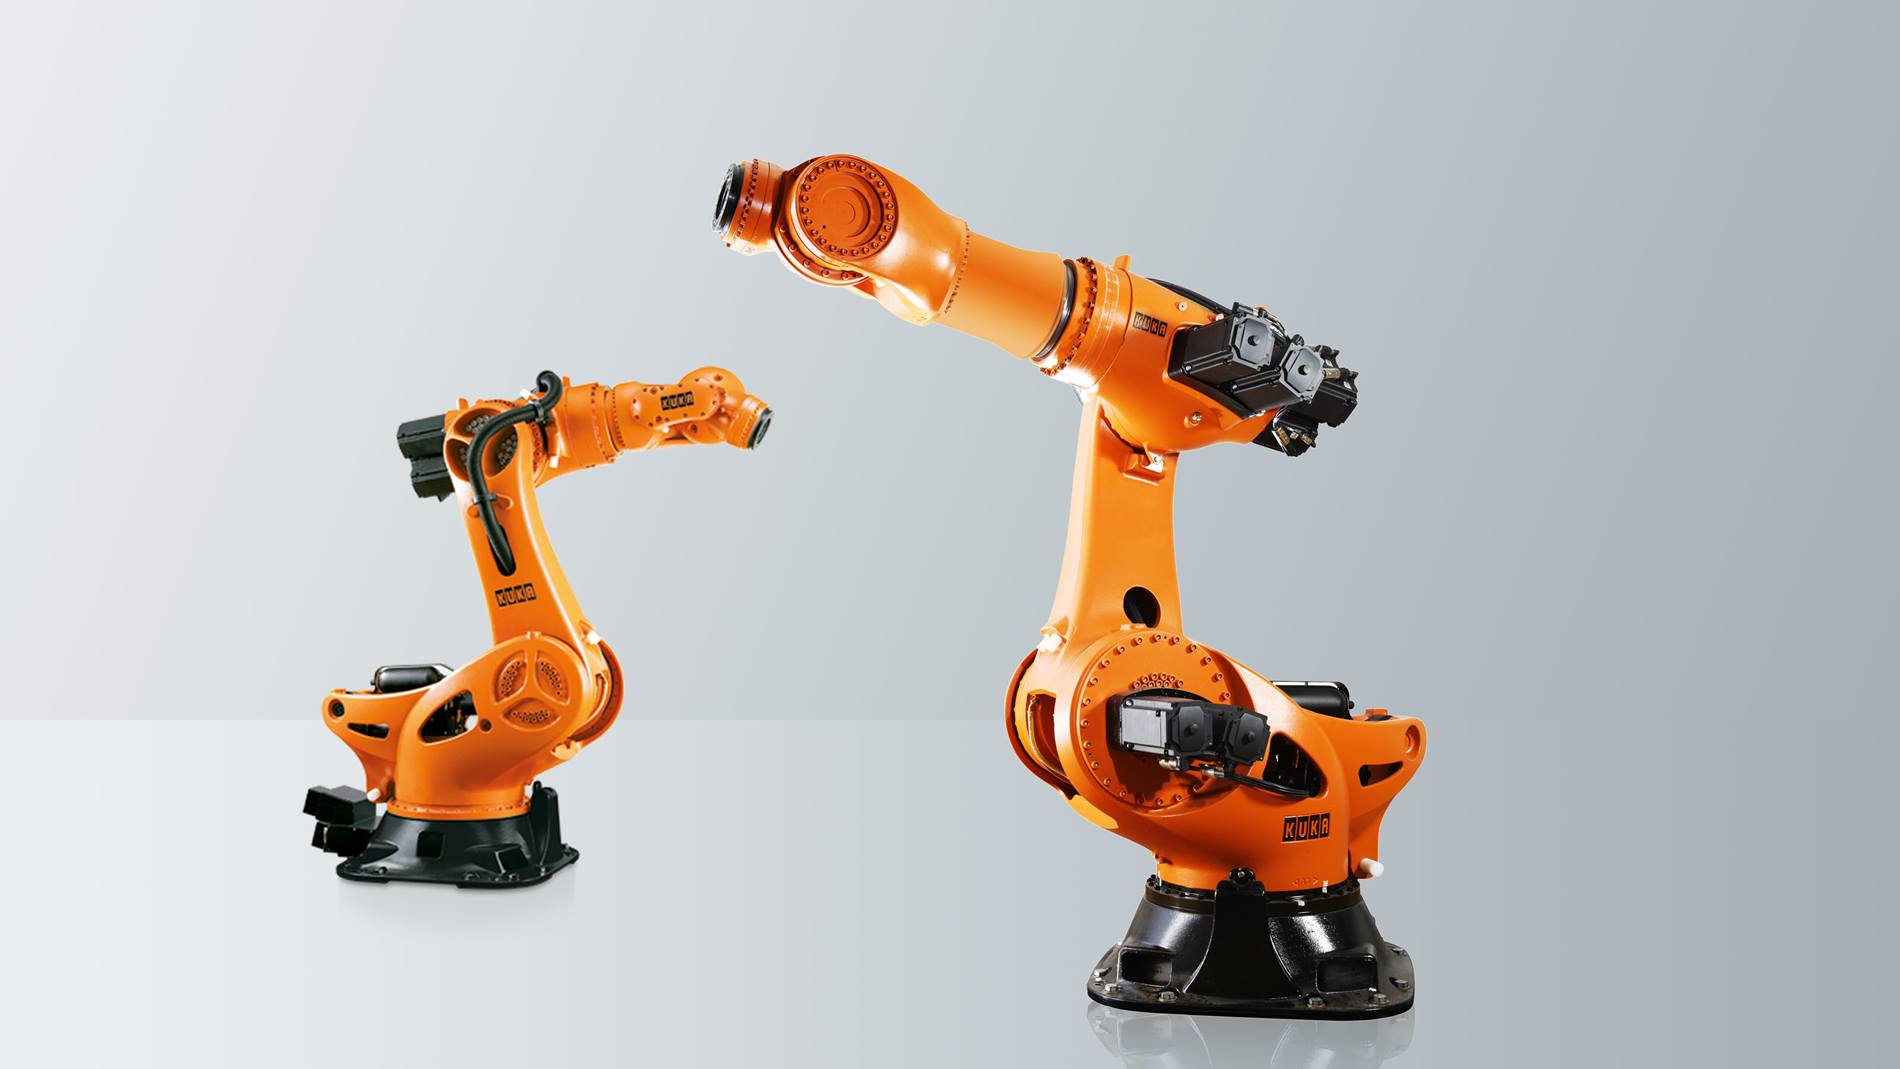
\includegraphics[width=0.60\textwidth]{Imagenes/modelo_3.jpg}
    \caption{Robot físico real.}
    \label{fig:etiqueta de la figura}
\end{figure}

\subsection{Modelo Físico}

Una vez seleccionado el sistema dinámico real a estudiar, se procedió a construir el modelo físico. En el cual, como primera instancia se habían considerado los 6 gdl del robot como se describe a continuación:

Se tienen 6 coordenadas generalizadas, y 6 grados de libertad del sistema real, una por cada articulación del robot. A las cuales, desde la articulación base hasta la articulación que hace rotar propiamente dicho al efector final, se las nombra como: \theta_1, \theta_2, \theta_3, \theta_4, \theta_5, \theta_6.

 \text{En donde, cada uno de estos gdl, describe un movimiento de vibración en los siguientes}\\
 \text{planos del espacio cartesiano tridimensional:}\\
\theta_1  ->  plano XY\\
\theta_2  ->  plano XZ\\
\theta_3  ->  plano XZ\\
\theta_4  ->  plano YZ\\
\theta_5  ->  plano XZ\\
\theta_6  ->  plano XY \text{ (rotación del efector final)}.\\

\subsection{Primer aproximación del modelo}

\begin{figure}[H]
    \centering
    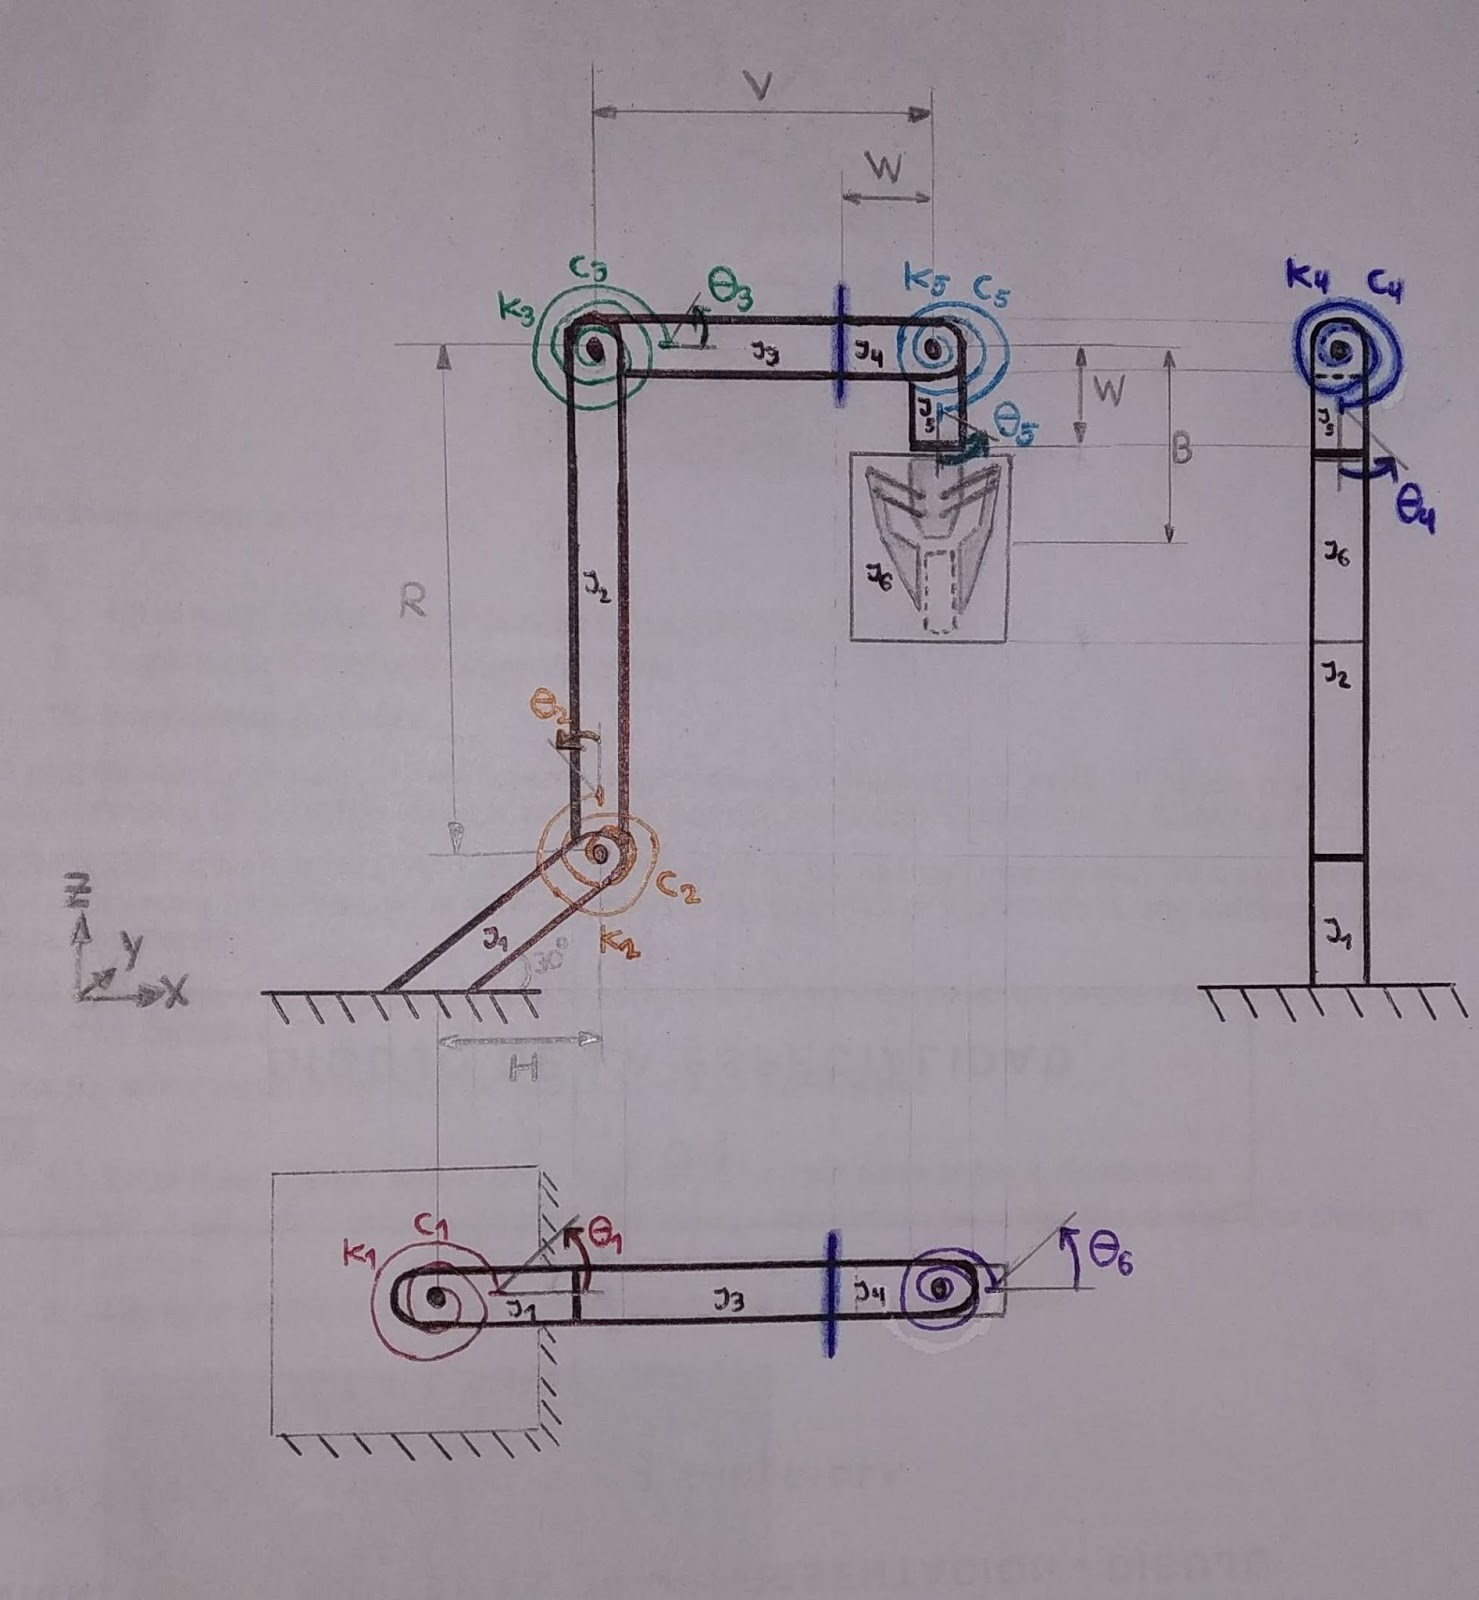
\includegraphics[width=0.60\textwidth]{Imagenes/modelo_4.jpg}
    \caption{Primer esquema del Sistema Dinámico [No se utiliza].}
    \label{fig:etiqueta de la figura}
\end{figure}

Este fue el primer modelo planteado pero luego se razonó que la complejidad del sistema superaba a los alcances previstos para el proyecto. Esta alta complejidad es debida al movimiento tridimensional producido por los múltiples gdl del sistema, ya que daría lugar a ecuaciones de movimiento demasiado grandes, e incluso se deberían considerar fuerzas de coriolis.

\text{Por ello, se optó por reducir la cantidad de gdl a 4, no considerando los gdl correspondientes a }\theta_1 \\ \text{ ni } \theta_4 \text{ mostrados en la figura anterior, y solo se toman a } \theta_2, \theta_3 \text{ y } \theta_5 \text{del plano XZ, y a } \theta_6 \text{ del plano XY.} \\
\text{Por lo que, con esta simplificación, para el estudio descrito a lo largo del artículo solo se tendrá en }\\ \text{cuenta el movimiento en el plano XZ, ya que el gld} \theta_6 \text{solo produce la rotación del efector final sobre} \\
\text{su mismo eje.}


\subsection{Modelo simplificado utilizado}

El modelo físico queda simplificado como se muestra en el siguiente esquema:

\begin{figure}[H]
    \centering
    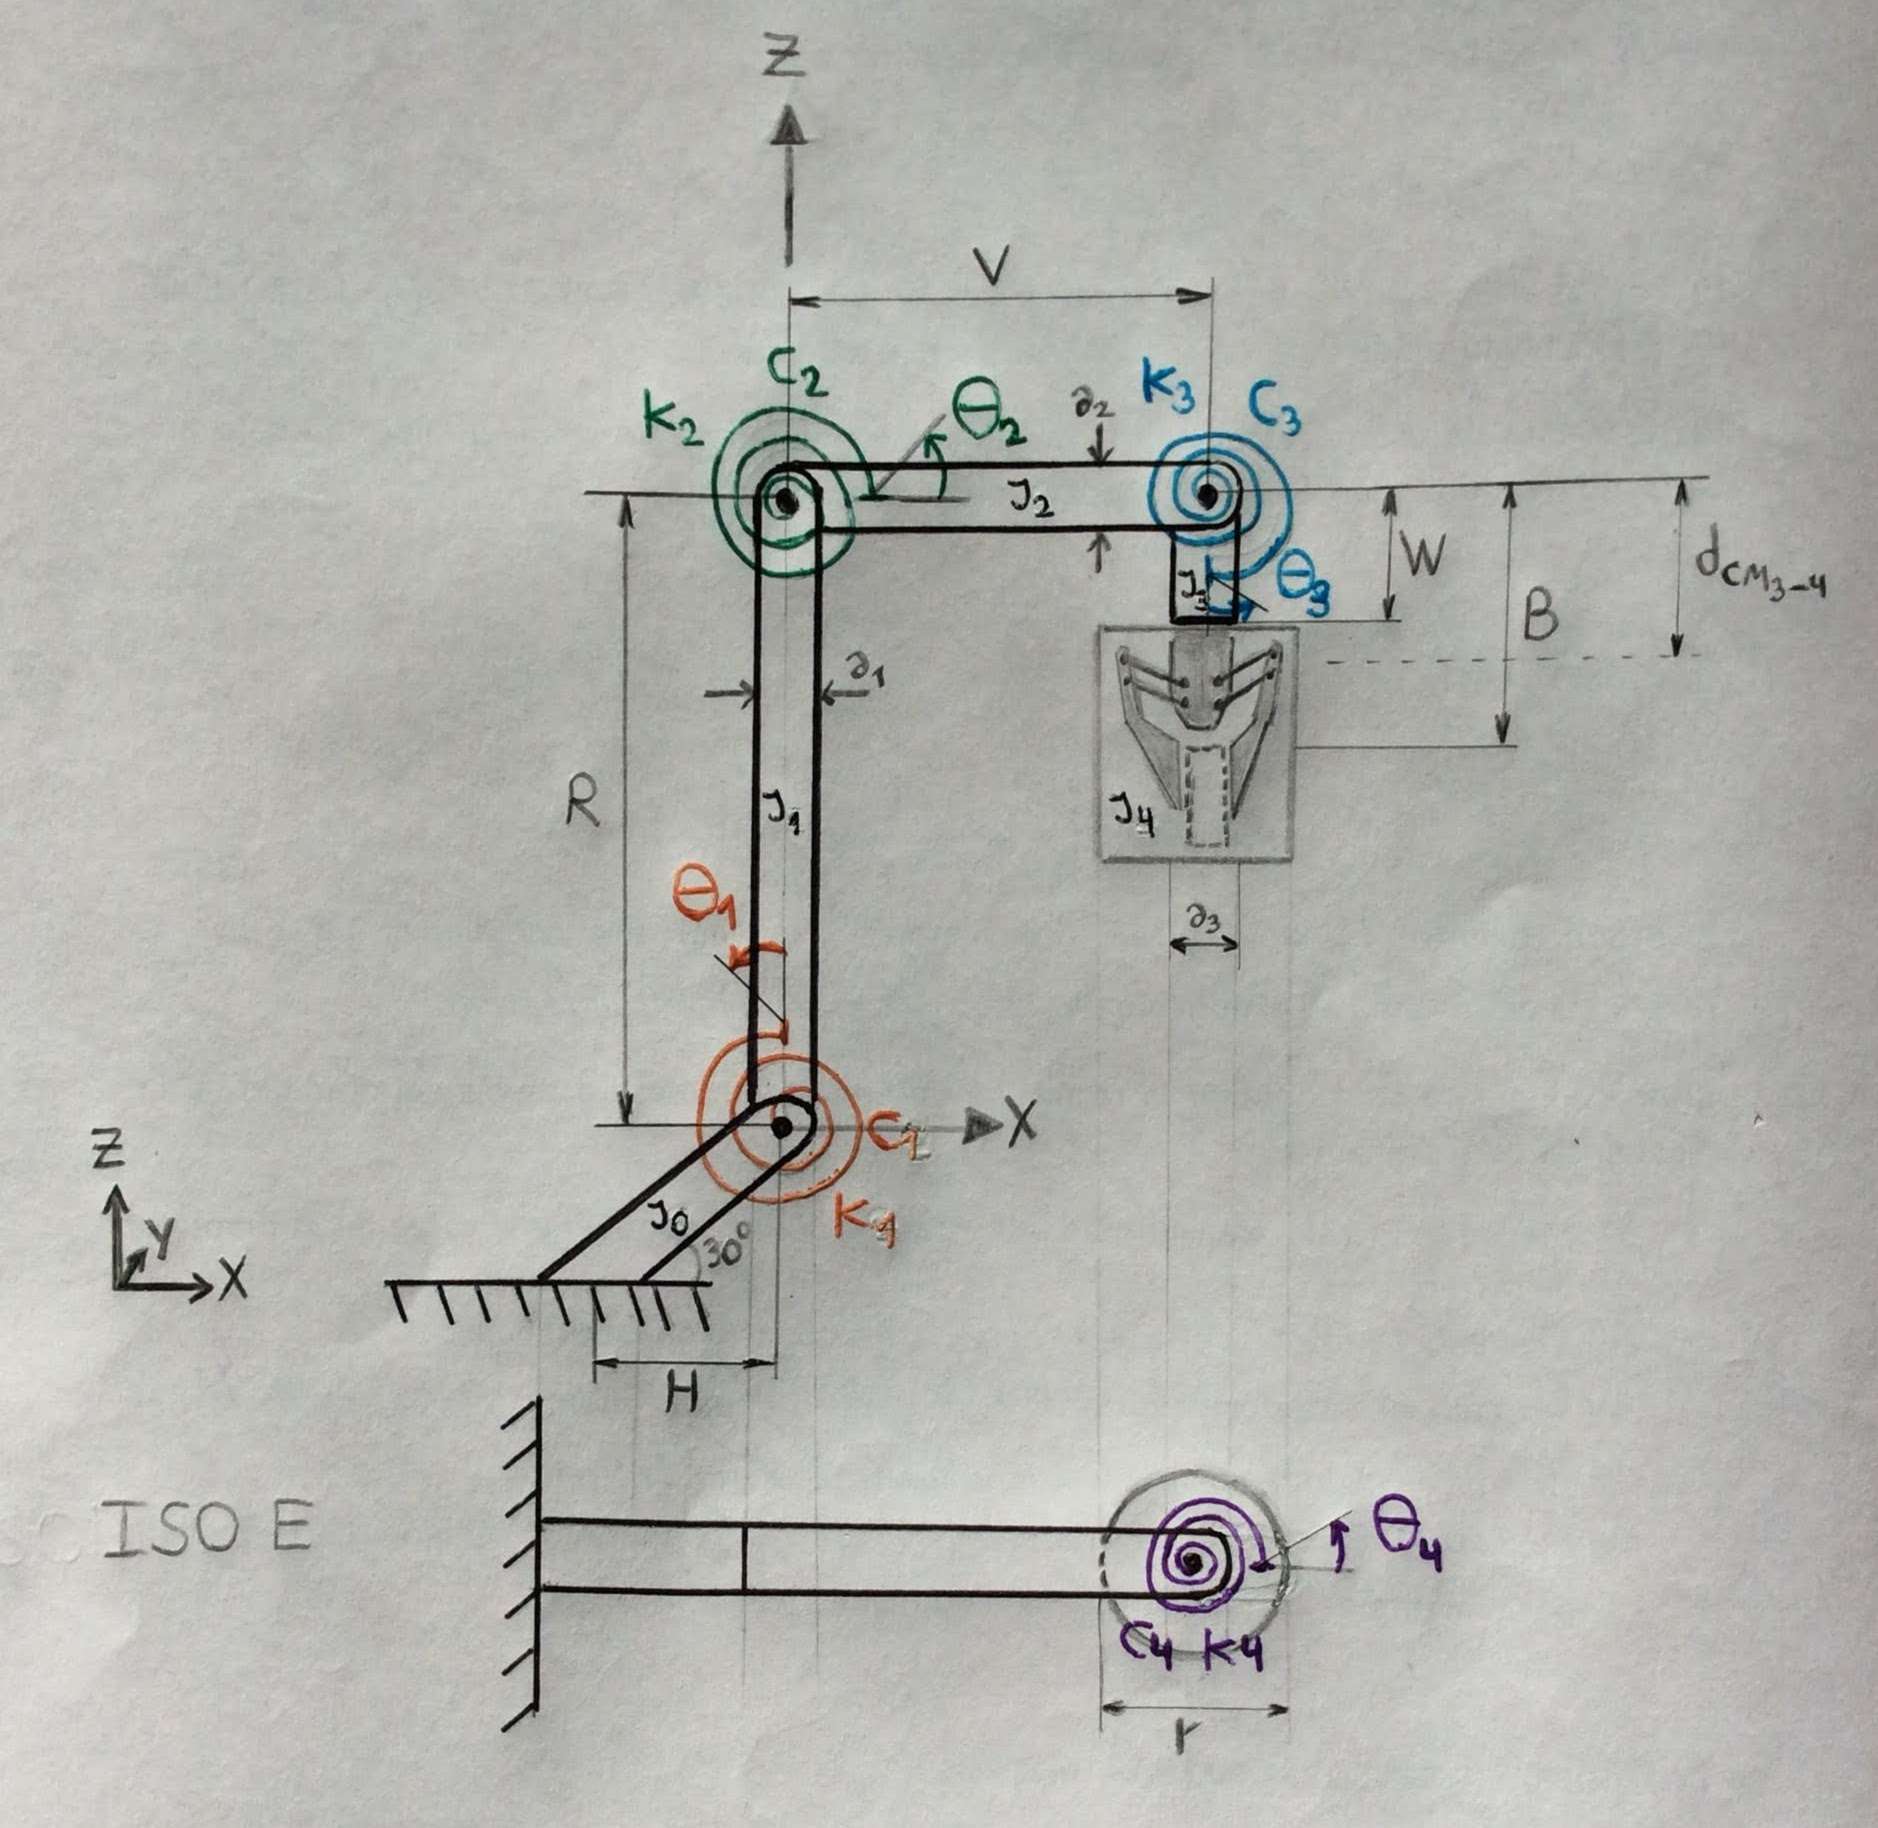
\includegraphics[width=0.60\textwidth]{Imagenes/modelo.jpg}
    \caption{Interpretación del robot físico real para su respectivo modelado.}
    \label{fig:etiqueta de la figura}
\end{figure}

Al plantear el modelo físico se decidió incorporar al robot un efector final genérico. En específico se muestra en el esquema el dibujo de una pinza robótica (Gripper), la cual puede estar o no sosteniendo un objeto a desplazar. La masa de dicho objeto, sumada a la masa del Efector Final constituyen la masa denominada: $m_4$.
Y siendo $dcm_3_4$ la distancia desde el centro de rotación de la articulación 3 hasta el centro de masa de la masa $m_4$.


Otra simplificación importante que se tiene en cuenta en el modelo, es la de considerar los ángulos como absolutos en el espacio, y no articulares como serían propiamente en el robot. Esto es también para facilitar el desarrollo de las ecuaciones en el modelo matemático.


\subsection{Masas implicadas en el modelo}

Masa total, incluyendo servomotores, sin efector final, y sin unidad de control: 4690kg\\
Masa estimada de la base fija empotrada: 690kg \\
Masa de cada uno de los 6 servomotores: 42kg.
[ (6servos*42kg)/4000kg = 0,063 ]  
 \\Se observa que la masa de los servomotores es insignificante respecto a la masa de todo el sistema, por lo que se considera la masa de cada motor como incluida en la masa de  tres primeras barras (ejes) del modelo del robot:\\

- Masa estimada de barra 0:	m_{0} =(4690kg - 690kg)/3partes = 1333kg\\

- Masa estimada de barra 1: m_{1} = 1333kg\\

- Masa estimada de barra 2: m_{2} = 800kg + (1333kg-800kg)/2 = 1067kg

[ 4690kg = 690kg + 2*1333kg + 1067kg + 267kg ]\\

- Masa estimada de barra 4 [Efector Final Genérico + Carga Genérica]:  310kg\\

Masa Neta (incluyendo efector final y carga):  5000kg

\subsection{Rigideces rotacionales de los Servomotores}

Luego de una extensa búsqueda en internet, se lograron encontrar los valores de las rigideces rotacionales k de los servomotores del robot Kuka:

\begin{figure}[H]
    \centering
    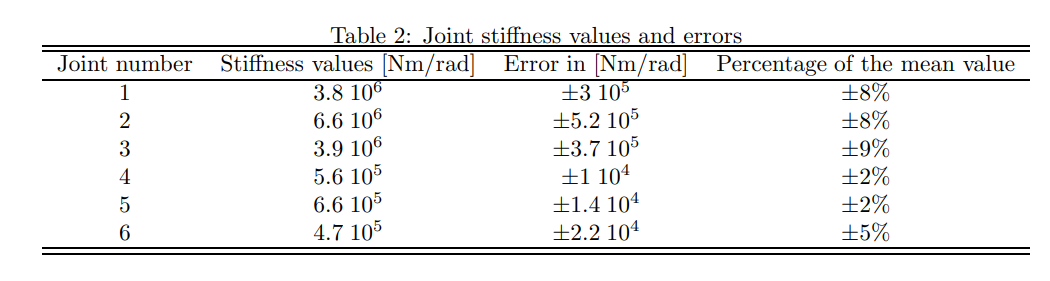
\includegraphics[width=0.60\textwidth]{Imagenes/ks.png}
    \caption{Fuente: https://hal.archives-ouvertes.fr/hal-00633095/document.}
    \label{fig:etiqueta de la figura}
\end{figure}

De los cuales solo se utilizaran los valores de las articulaciones 2, 3, 5 y 6, reescritos a continuación:
\\$k_1$ = 6,6 x106 Nm/rad
\\$k_2$ = 3,9 x106 Nm/rad
\\$k_3$ = 6,6 x105 Nm/rad
\\$k_4$ = 4,7 x105 Nm/rad

\subsection{Amortiguamientos rotacionales de los servomotores}

Luego de una extensa búsqueda en internet, no se pudieron encontrar por ningún lado los 
valores de los amortiguamientos rotacionales c de los servomotores del robot kuka.

Por lo que los amortiguamientos se obtuvieron al final de la simulación utilizando la función lsqr de MATLAB (método de los mínimos cuadrados) ya que con la matriz Keq y Meq obtuvimos la matriz Cmodal, aplicando las ecuaciones correspondientes obtuvimos C y comparamos los valores obtenidos con los del modelo.
$c_1$ = 1.2044  x108   Nms/rad
$c_2$ = 0.4118  x108   Nms/rad
$c_3$ = 0.1289  x108   Nms/rad
$c_4$ = - 0.0005  x108 Nms/rad

Se utilizaron amortiguamientos $\zeta$ = [ 0.02; 0.03; 0.04; 0.043 ], ya con Meq y Keq se resolvió el problema a través del método de descomposición modal para obtener la solución del sistema.

Comparándolo con una investigación similar: Vibration damping control of robot arm intended for service application in human environment.
Se pudo observar que el $\zeta$=0.0249  considerando el brazo robótico solo como 2 masas, por lo cual se puede asegurar que los valores de amortiguamiento son cercanos a los experimentales.


%%%%%%%%%%%%%%%%%%%%%%%%%%%%%%%%%%%%%%%%
\section{Coordenadas Generalizadas}
%%%%%%%%%%%%%%%%%%%%%%%%%%%%%%%%%%%%%%%%

\subsection{Coordenadas del centro de masa de cada barra considerada (barras 1,2 y 3-4)}

\begin{flalign*}
    &X_c_1 = -\frac{R}{2}sen\theta_1&
    &Z_c_1 = \frac{R}{2}cos\theta_1& \\
    &X_c_2 = -Rsen\theta_1 + \frac{V}{2}cos\theta_2&
    &Z_c_2 = Rcos\theta_1 + \frac{V}{2}sen\theta_2& \\
    &X_c_3_4 = - Rsen\theta_1 + Vcos\theta_2 + dcm_3_4sen\theta_3&
    &Z_c_3_4 = Rcos\theta_1 + Vsen\theta_2 - dcm_3_4cos\theta_3&
\end{flalign*}



\subsection{Velocidades del centro de masa de cada barra considerada (barras 1,2 y 3-4)}

\begin{flalign*}
    &\dot{X}_c_1 = -\frac{R}{2}\dot{\theta_1}sen\theta_1&
    &\dot{Z}_c_1 = \frac{R}{2}\dot{\theta_1}cos\theta_1& \\
    &\dot{X}_c_2 = -R\dot{\theta_1}sen\theta_1 + \frac{V}{2}\dot{\theta_2}cos\theta_2&
    &\dot{Z}_c_2 = R\dot{\theta_1}cos\theta_1 + \frac{V}{2}\dot{\theta_2}sen\theta_2& \\
    &\dot{X}_c_3_4 = - R\dot{\theta_1}sen\theta_1 + V\dot{\theta_2}cos\theta_2 + dcm_3_4\dot{\theta_3}sen\theta_3&
    &\dot{Z}_c_3_4 = R\dot{\theta_1}cos\theta_1 + V\dot{\theta_2}sen\theta_2 - dcm_3_4\dot{\theta_3}cos\theta_3&
\end{flalign*}

\noindent
\text{donde }{dcm_3_4 = \frac{m_3\frac{W}{2} + m_4B}{m_3+m_4}

\subsection{Momentos de Inercia}
\begin{flalign*}
    &J_1_Y = \frac{1}{12}m_1(R^2 + d_1^2)&
    &J_2_Y = \frac{1}{12}m_2(V^2 + d_2^2)&\\
    &J_4_Z = \frac{1}{2} m_4r^2&
    &J_3_4_Y = [J_3_Y + m_3(dcm_3_4 - \frac{W}{2})^2] + [J_4_Y + m_4(B - dcm_3_4)^2] &
\end{flalign*}

%%%%%%%%%%%%%%%%%%%%%%%%%%%%%%%%%%%%%%%%
\section{Formulación de las ecuaciones de movimiento}
%%%%%%%%%%%%%%%%%%%%%%%%%%%%%%%%%%%%%%%%

\subsection{Energía cinética total}
\begin{flalign*}
    &T = \frac{1}{2}m_1[\dot{X_c_1}^2 + \dot{Z_c_1}^2] + \frac{1}{2}m_2[\dot{X_c_2}^2 + \dot{Z_c_2}^2] + \frac{1}{2}(m_3+m_4)[\dot{X_c_3_4}^2 + \dot{Z_c_3_4}^2] + \frac{1}{2}J_1_Y\dot{\theta_1}^2& \\
    &+\frac{1}{2}J_2_Y\dot{\theta_2}^2+\frac{1}{2}J_3_4_Y\dot{\theta_3}^2 + \frac{1}{2}J_4_Z\dot{\theta_4}^2&
\end{flalign*}

\subsection{Energía disipada total}
\begin{flalign*}
    &D =\frac{1}{2}[c_1\dot{\theta_1}^2 + c_2(\dot{\theta_2}-\dot{\theta_1})^2 + c_3(\dot{\theta_3}-\dot{\theta_3})^2 + c_4\dot{\theta_4}^2]&
\end{flalign*}

\subsection{Energía potencial total}
\begin{flalign*}
&U = \frac{1}{2}[k_1\theta_1^2 + k_2(\theta_2 - \theta_1)^2 + k_3(\theta_3 - \theta_2)^2 + k_4\theta_4^2] + [m_1g\frac{R}{2}(1 + cos\theta_1) + m_2g[R(1+cos\theta1) + & \\ 
&(m_3+m_4)g(R-dcm_3_4)(1+cos\theta_1)] + [m_2g\frac{V}{2}(1 + sen\theta_2)] + (m_3+m_4)gV(1+sen\theta_2)&\\
&+(m_3+m_4)gdcm_3_4(1-cos\theta_3)&
\end{flalign*}

%%%%%%%%%%%%%%%%%%%%%%%%%%%%%%%%%%%%%%%%
\section{Desarrollo de las ecuaciones de Lagrange}
%%%%%%%%%%%%%%%%%%%%%%%%%%%%%%%%%%%%%%%%

\subsection{Para \theta_1}

\begin{flalign*}
    &\frac{\partial(U)}{\partial(\theta_1)} = \theta_1[k_1 + k_2 - m_1g\frac{R}{2} - (m_3 + m_4)g(R-dcm_3_4) + \theta_2(-k_2)]&
\end{flalign*}

\begin{flalign*}
    &\frac{\partial(D)}{\partial(\dot{\theta_1})} = \dot{\theta_1}(c_1 + c_2) + \dot{\theta_2}(-c_2)&
\end{flalign*}

\begin{flalign*}
    &\frac{d(T)}{dt(\dot{\theta_1})} = J_1_Y\ddot{\theta_1} +  \ddot{\theta_1}(m_1)\frac{R^2}{4} + \frac{1}{2}m_2[ 2R^2\ddot{\theta_1} -V\ddot{\theta_2}R(cos\theta_2sen\theta_1 - cos\theta_1sen\theta_2)] + &\\ &\frac{1}{2}(m_3+m_4)[2R^2\ddot{\theta_4} - [2dcm_3_4\ddot{\theta_3}Rsen\theta_1sen\theta_3 + 2\ddot{\theta_2}VRcos\theta_2sen\theta_1 - 2dcm_3_4\ddot{\theta_3}Rcos\theta_1cos\theta_3]]&
\end{flalign*}

\begin{flalign*}
    &\frac{\partial(T)}{\partial(\theta_1)} = -\frac{1}{2}m_2VR\dot{\theta_1}\dot{\theta_2}(sen\theta_2sen\theta_1 - cos\theta_2cos\theta_1) -\frac{1}{2}(m_3+m_4)[ 2\dot{\theta_1}dcm_3_4\dot{\theta_3}Rcos\theta_1sen\theta_3 +&\\
    &(2\dot{\theta_1}\dot{\theta_2}VRsen\theta_2 - 2\dot{\theta_1} dcm_3_4\dot{\theta_3}Rcos\theta_3)sen\theta_1 + 2\dot{\theta_1}\dot{\theta_2}VRcos\theta_2cos\theta_1 ]&
\end{flalign*}

\subsection{Para \theta_2}

\begin{flalign*}
    &\frac{\partial(U)}{\partial(\theta_2)} = \theta_1(-k_2) + \theta_2(k_2 + k_3) + \theta_3(-k_3) + m_2g\frac{V}{2} + (m_3+m_4)gV&
\end{flalign*}

\begin{flalign*}
    &\frac{\partial(D)}{\partial(\dot{\theta_2})} = \dot{\theta_1}(-c_2) + \dot{\theta_2}(c_2+c_3) + \dot{\theta_3}(-c_3) &
\end{flalign*}

\begin{flalign*}
    &\frac{d(T)}{dt(\dot{\theta_2})} = J_2_Y*\ddot{\theta_2}(m_2\frac{V^2}{4}) + \ddot{\theta_1}[ -\frac{V}{2}R(cos\theta_2sen\theta_1 - cos\theta_1sen\theta_2)] + \frac{1}{2}(m_3+m_4)[2V^2\ddot{\theta_2} +&\\ &2Vdcm_3_4\ddot{\theta_3}cos\theta_2sen\theta3 - [2\ddot{\theta_1}VRcos\theta2sen\theta1 + (2Vdcm_3_4\ddot{\theta_3}cos\theta3 - 2\ddot{\theta_1}VRcos\theta1)sen\theta2] ]  &
\end{flalign*}

\begin{flalign*}
    &\frac{\partial(T)}{\partial(\theta_2)} = \frac{1}{2}m_2\dot{\theta_1}\theta2VR(sen\theta1sen\theta2 + cos\theta1cos\theta2) - \frac{1}{2}(m_3+m_4)[2\dot{\theta_2}Vdcm_3_4\dot{\theta_3}sen\theta2sen\theta3 -& \\ & (2\dot{\theta_1}\dot{\theta_2}VRsen\theta1sen\theta2 - (2\dot{\theta_2}Vdcm_3_4\dot{\theta_3}cos\theta2cos\theta3 - 2\dot{\theta_1}\dot{\theta_2}VRcos\theta1cos\theta2))]&
\end{flalign*}

\subsection{Para \theta_3}

\begin{flalign*}
    &\frac{\partial(U)}{\partial(\theta_3)} = k_3(\theta3- \theta2) + (m_3+m_4)gdcm_3_4sen\theta3&
\end{flalign*}

\begin{flalign*}
    &\frac{\partial(D)}{\partial(\dot{\theta_3})} = \dot{\theta_2}(-c_3) + \dot{\theta_3}(c_3) &
\end{flalign*}

\begin{flalign*}
    &\frac{d(T)}{dt(\dot{\theta_3})} = J_3_4_Y\ddot{\theta_3} + \frac{1}{2}(m_3+m_4)[2(dcm_3_4)^2\ddot{\theta_3} - (2dcm_3_4\ddot{\theta_1}Rsen\theta1 - 2\ddot{\theta_2}Vdcm_3_4cos\theta2)sen\theta3 + &\\ &2\ddot{\theta_2}Vdcm_3_4cos\theta3sen\theta2 + 2dcm_3_4\ddot{\theta_1}Rcos\theta1cos\theta3] &
\end{flalign*}

\begin{flalign*}
    &\frac{\partial(T)}{\partial(\theta_3)} = \frac{1}{2}(m_3+m_4)[2\dot{\theta_2}Vdcm_3_4\dot{\theta_3}sen\theta3sen\theta2 + 2\dot{\theta_1}dcm_3_4\dot{\theta_3}Rcos\theta1sen\theta3 -&\\ 
    & (2\dot{\theta_1}dcm_3_4\dot{\theta_3}Rcos\theta3sen\theta1 - 2\dot{\theta_2}Vdcm_3_4\dot{\theta_3}cos\theta3cos\theta2)]&
\end{flalign*}

\subsection{Para \theta_4}

\begin{flalign*}
    &\frac{\partial(U)}{\partial(\theta_4)} = \theta4(k_4)&
\end{flalign*}

\begin{flalign*}
    &\frac{\partial(D)}{\partial(\dot{\theta_4})} = \dot{\theta_4}(c_4)&
\end{flalign*}

\begin{flalign*}
    &\frac{d(T)}{dt(\dot{\theta_4})} =  J_4_Z\ddot{\theta_4}&
\end{flalign*}

\begin{flalign*}
    &\frac{\partial(T)}{\partial(\theta_4)} = 0&
\end{flalign*}

%%%%%%%%%%%%%%%%%%%%%%%%%%%%%%%%%%%%%%%%
\section{Reducción de las ecuaciones de Lagrange}
%%%%%%%%%%%%%%%%%%%%%%%%%%%%%%%%%%%%%%%%

\noindent
\text{Se realizó una simplificación para todos los Grados de Libertad:} {sen\theta_i = 0} \text{ y } {cos\theta_i = 1}. \\
\text{También por ortogonalidad } {\dot{\theta_i}\dot{\theta_j} = 0}. \\ 

\noindent
\text{Cabe destacar que en primera instancia se considero una fuerza no restitutiva en nuestro modelo} \\
\text{e impedía la linealización de las ecuaciones. Por eso se suprimió para linealizar las ecuaciones} \\
\text{equivalentes.}

\subsection{C equivalente}   
\begin{equation}
\begin{bmatrix}
c_1+c_2 & -c_2 & 0 & 0\\
-c_2 & c_2+c_3 & -c_3 & 0\\
0 & -c_3 & c_3 & 0\\
0 & 0 & 0 & c_4
\end{bmatrix}
\end{equation} 

\subsection{K equivalente}   
\begin{equation}
\begin{bmatrix}
k_1+k_2-m_1g\frac{R}{2}-m_2gR-(m_3+m_4)g(R-dcm_3_4) & -k_2 & 0 & 0\\
-k_2 & k_2+k_3 & -k_3 & 0\\
0 & -k_3 & (m_3+m_4)gdcm_3_4 + k_3 & 0\\
0 & 0 & 0 & k_4
\end{bmatrix}
\end{equation}

\subsection{M equivalente}   
\begin{equation}
\begin{bmatrix}
J_1_Y + m1\frac{R^2}{4}+m_2R^2 & 0 & (m_3+m_4)(Rdcm_3_4) & (m3+m4)R^2\\
0 &J_2_Y+(m_2\frac{V^2}{2})+(V^2)(m_3+m_4) &-(m_3+m_4)Vdcm_3_4 & 0 \\
(m_3+m_4)(Rdcm_3_4) & -(m_3+m_4)Vdcm_3_4 & J_3_4_Y+(m_3+m_4)*(dcm_3_4^2) & 0\\
0 & 0 & 0 & J_4_Z
\end{bmatrix}
\end{equation}

%%%%%%%%%%%%%%%%%%%%%%%%%%%%%%%%%%%%%%%%
\section{Modelo Matemático}
%%%%%%%%%%%%%%%%%%%%%%%%%%%%%%%%%%%%%%%%   

Al sustituir las variables de las matrices por sus valores numéricos:

\begin{figure}[H]
    \centering
    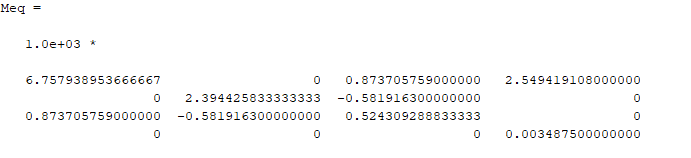
\includegraphics[width=0.90\textwidth]{Imagenes/meq.png}
    \caption{Matriz equivalente de masas Meq.}
    \label{fig:etiqueta de la figura}
\end{figure}

\begin{figure}[H]
    \centering
    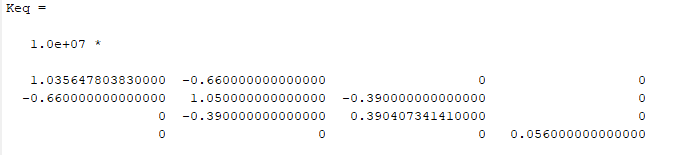
\includegraphics[width=0.90\textwidth]{Imagenes/keq.png}
    \caption{Matriz equivalente de rigideses Keq.}
    \label{fig:etiqueta de la figura}
\end{figure}

\begin{figure}[H]
    \centering
    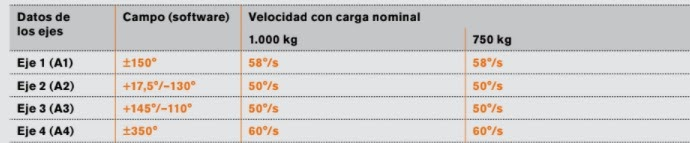
\includegraphics[width=0.90\textwidth]{Imagenes/cei.jpg}
    \caption{Valores de CI (condiciones iniciales).}
    \label{fig:etiqueta de la figura}
\end{figure}

Como criterio para las condiciones iniciales de nuestro problema, se simularán con distintos valores la velocidad inicial máxima dada por el fabricante, 58°/s para el 1° eje, 50°/s para el 2°, 50°/s para el 3°, y 60°/s para el 4, en unidades de sistema internacional corresponden a:
$V_0$=[1.0123, 0.873, 0.873, 1.0472] rad/s donde cada posición corresponde a cada eje correspondiente. En todos los casos la posición inicial $X_0$=[0, 0, 0, 0]

%%%%%%%%%%%%%%%%%%%%%%%%%%%%%%%%%%%%%%%%
\section{Métodos utilizados para la resolución de las ecuaciones de movimiento}
%%%%%%%%%%%%%%%%%%%%%%%%%%%%%%%%%%%%%%%%

\subsection{Método de descomposición modal}

Es un método utilizado para la resolución de sistemas de N grados de libertad, donde se trabaja con N ecuaciones diferenciales ordinarias de segundo orden acopladas entre sí.

Los desplazamientos asociados a los grados de libertad se expresan como una combinación lineal de los modos normales del sistema. Esta transformación lineal desacopla el sistema de ecuaciones diferenciales original, de manera de obtener un sistema de N ecuaciones diferenciales de segundo orden desacoplado.

%%%%%%%%%%%%%%%%%%%%%%%%%%%%%%%%%%%%%%%%
\section{Solución del modelo matemático}
%%%%%%%%%%%%%%%%%%%%%%%%%%%%%%%%%%%%%%%%

Para el cálculo de las frecuencias naturales de vibración primero fue necesario calcular los autovalores y autovectores, para se utilizó la función de MATLAB “eig()”, la cual nos da los autovalores y autovectores del sistema normalizados usando la matriz de masas y la matriz de rigidez. Los autovectores se agrupan por columnas en una matriz, que llamamos “Matriz Modal Nomal”:

\begin{figure}[H]
    \centering
    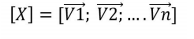
\includegraphics[width=0.40\textwidth]{Imagenes/e0.png}
    }
\end{figure}

Siendo $V_n$ cada uno de los vectores propios normalizados. En el caso del modelo los vectores propios obtenidos fueron:

\begin{figure}[H]
    \centering
    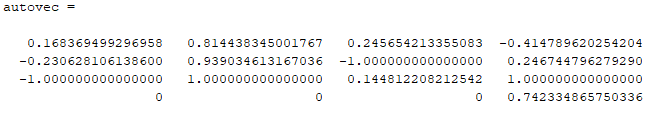
\includegraphics[width=0.90\textwidth]{Imagenes/e1.png}
    }
\end{figure}

Una vez obtenido los autovalores, aplicaremos la raíz cuadrada a cada uno de los mismos para obtener la frecuencia natural de vibración ($w_n_i$) relacionada con cada modo, siendo estas:

\noindent
$w_n_1$ = 1.112 x102 rad/s
\\$w_n_2$ = 0.187 x102 rad/s
\\$w_n_3$ = 0.715 x102 rad/s
\\$w_n_4$ = 4.007 x102 rad/s


Para obtener la matriz de amortiguamiento C, como se conoce las frecuencias naturales de vibración circulares y, la relación de amortiguamiento crítico( $\zeta$ ), para todos los modos de vibración considerados es posible formar la siguiente matriz diagonal:

\begin{figure}[H]
    \centering
    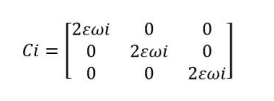
\includegraphics[width=0.40\textwidth]{Imagenes/e2.png}
    }
\end{figure}

Siendo $\varepsilon$ el valor de amortiguamiento y $\omega_i$ cada una de las frecuencias naturales circulares de vibración

Para poder obtener finalmente la matriz de amortiguamiento C, se realiza la siguiente operación:

\begin{figure}[H]
    \centering
    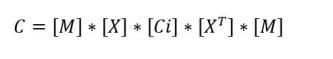
\includegraphics[width=0.40\textwidth]{Imagenes/e3.png}
    }
\end{figure}

Siendo M la matriz de Masa equivalente de la ecuación de movimiento, X matriz modal normal y $X^T$ su transpuesta

Para obtener las ecuaciones desacopladas partimos de la EDO que modela a nuestro sistema

\begin{figure}[H]
    \centering
    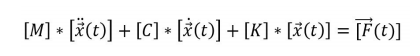
\includegraphics[width=0.60\textwidth]{Imagenes/e4.png}
    }
\end{figure}

Donde F(t)=0.
Considerando que x(t) es una combinación de la matriz modal norma.

\begin{figure}[H]
    \centering
    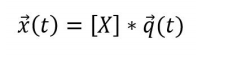
\includegraphics[width=0.40\textwidth]{Imagenes/e5.png}
    }
\end{figure}

Teniendo en cuenta que la matriz de amortiguamiento proporcional que se obtuvo de Ci y haciendo los reemplazos correspondientes, la ecuación de movimiento re expresada nos queda:

\begin{figure}[H]
    \centering
    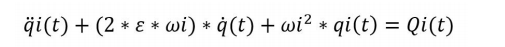
\includegraphics[width=0.60\textwidth]{Imagenes/e6.png}
    }
\end{figure}

Siendo [ $\omega_i_2$ ] una matriz diagonal que contiene cada una de las frecuencias naturales de vibración del sistema. 
De esta forma obtenemos un sistema de ecuaciones totalmente desacoplado, donde cada ecuación depende de su constante generalizada $q_i$(t). Expresamos la respuesta de la ecuación dada por la bibliografía:


\begin{figure}[H]
    \centering
    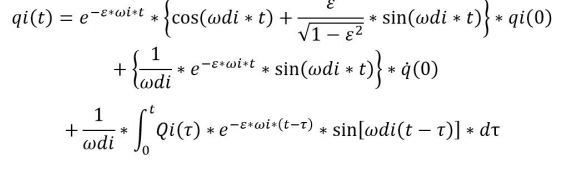
\includegraphics[width=0.80\textwidth]{Imagenes/e7.png}
    }
\end{figure}

Donde:
\begin{figure}[H]
    \centering
    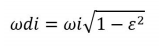
\includegraphics[width=0.30\textwidth]{Imagenes/e8.png}
    }
\end{figure}

\begin{figure}[H]
    \centering
    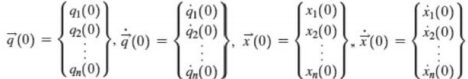
\includegraphics[width=0.80\textwidth]{Imagenes/e9.png}
    }
\end{figure}

Estas son las condiciones iniciales expresadas en coordenadas generalizadas

Con este método podemos pasar de “Coordenadas Generalizadas” (q(t)) a “Coordenadas geométricas” (x(t)), se obtiene la respuesta de cada uno de los grados de libertad del sistema en el tiempo.

La bibliografía consultada para este procedimiento fue: Daniel J. Inman Engineering Vibration, U4 Multiple Degree of freedom Systems- U4.3 Modal Análisis

%%%%%%%%%%%%%%%%%%%%%%%%%%%%%%%%%%%%%%%%
\section{Resultados}
%%%%%%%%%%%%%%%%%%%%%%%%%%%%%%%%%%%%%%%%

\subsection{Para $X_0$=[0, 0, 0, 0] y $V_0$=[1.0123, 0, 0, 0] y considerando que no tenemos carga adicional en el efector final ($m_4$= 310kg - peso del brazo)}
\begin{figure}[H]
    \centering
    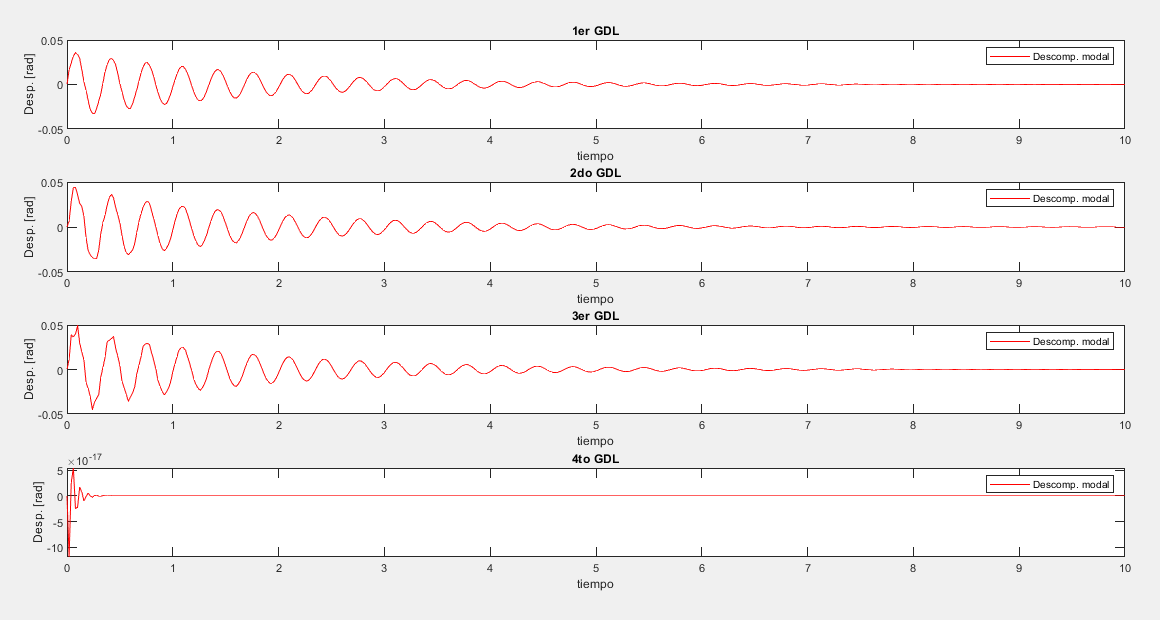
\includegraphics[width=0.90\textwidth]{Imagenes/r1.png}
    \caption{Gráfica de posición}
    \label{fig:etiqueta de la figura}
\end{figure}

\begin{figure}[H]
    \centering
    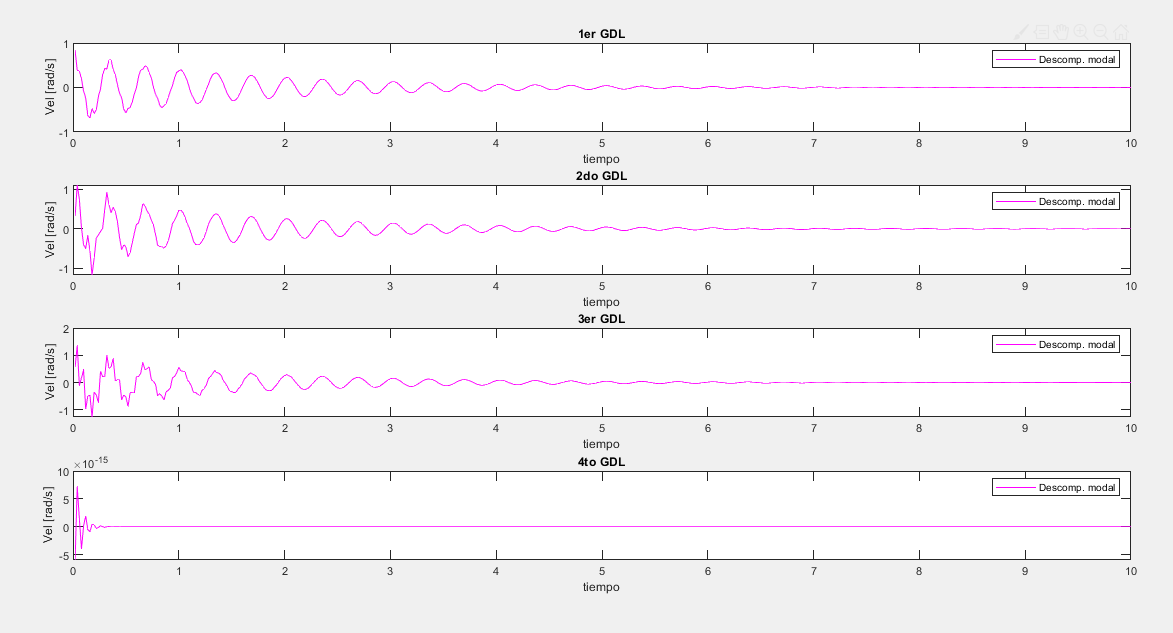
\includegraphics[width=0.90\textwidth]{Imagenes/r2.png}
    \caption{Gráfica de velocidad}
    \label{fig:etiqueta de la figura}
\end{figure}

\begin{figure}[H]
    \centering
    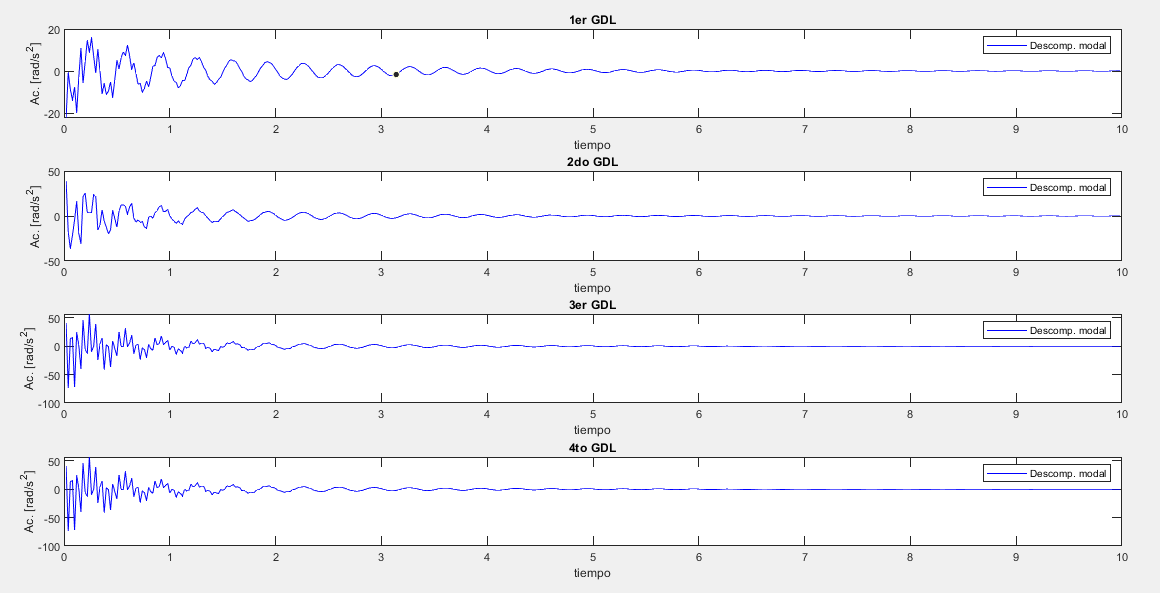
\includegraphics[width=0.90\textwidth]{Imagenes/r3.png}
    \caption{Gráfica de aceleración}
    \label{fig:etiqueta de la figura}
\end{figure}


\subsection{Para $X_0$=[0, 0, 0, 0] y $V_0$ =[0, 0.873, 0, 0] y considerando que no tenemos carga adicional en el efector final ($m_4$= 310kg):}
\begin{figure}[H]
    \centering
    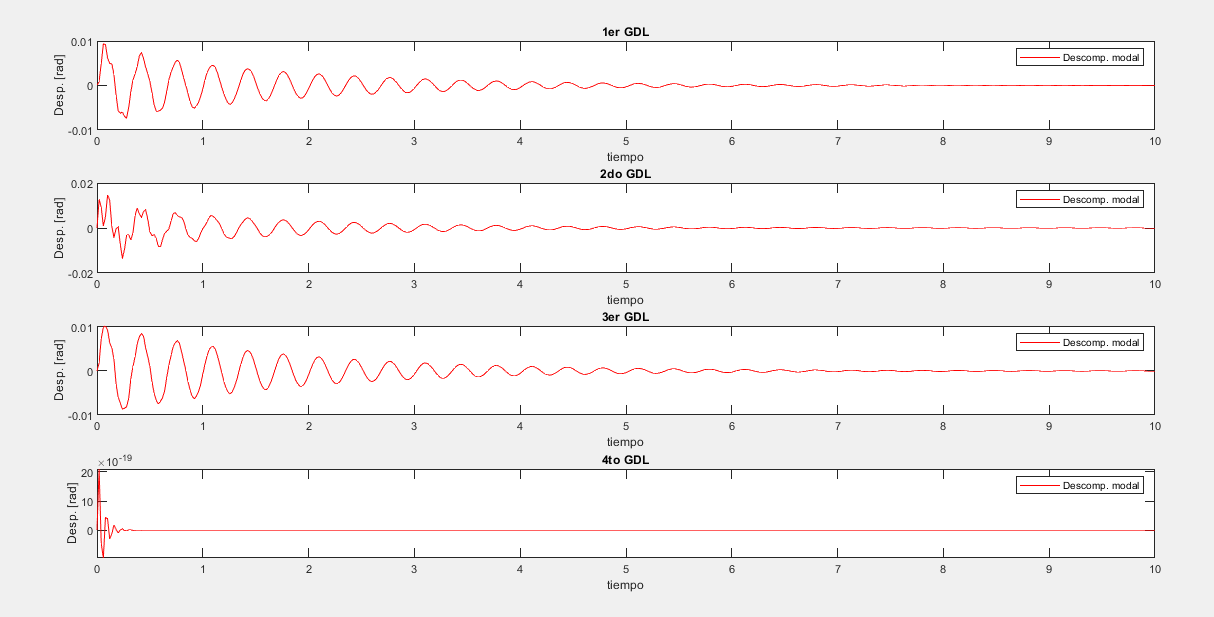
\includegraphics[width=0.90\textwidth]{Imagenes/r4.png}
    \caption{Gráfica de posición}
    \label{fig:etiqueta de la figura}
\end{figure}

\begin{figure}[H]
    \centering
    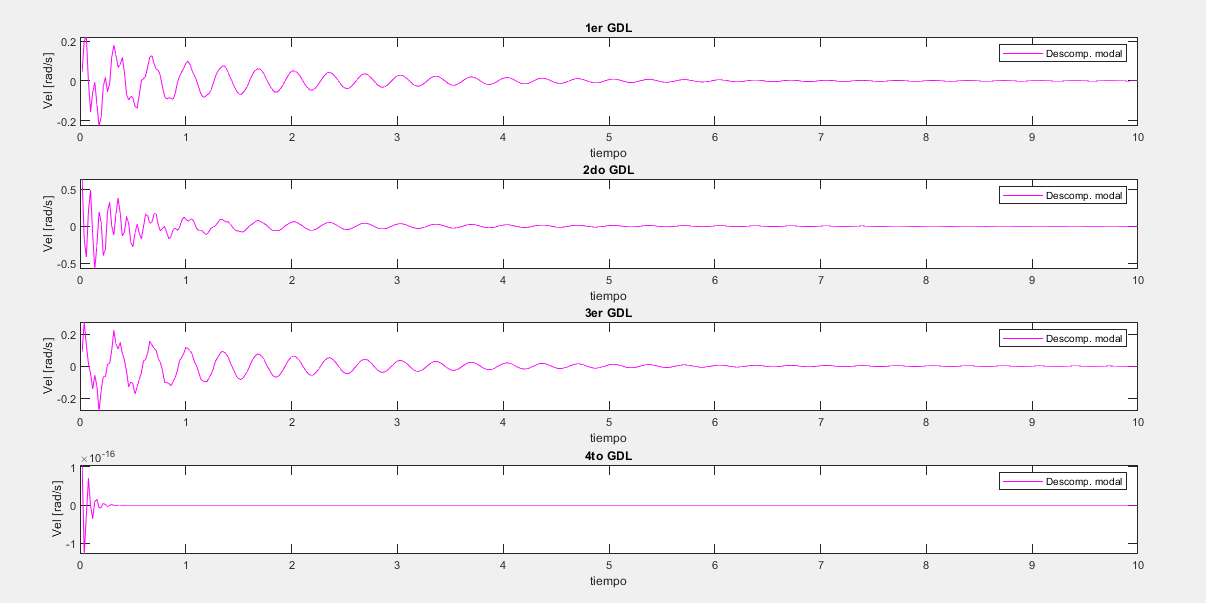
\includegraphics[width=0.90\textwidth]{Imagenes/r5.png}
    \caption{Gráfica de velocidad}
    \label{fig:etiqueta de la figura}
\end{figure}

\begin{figure}[H]
    \centering
    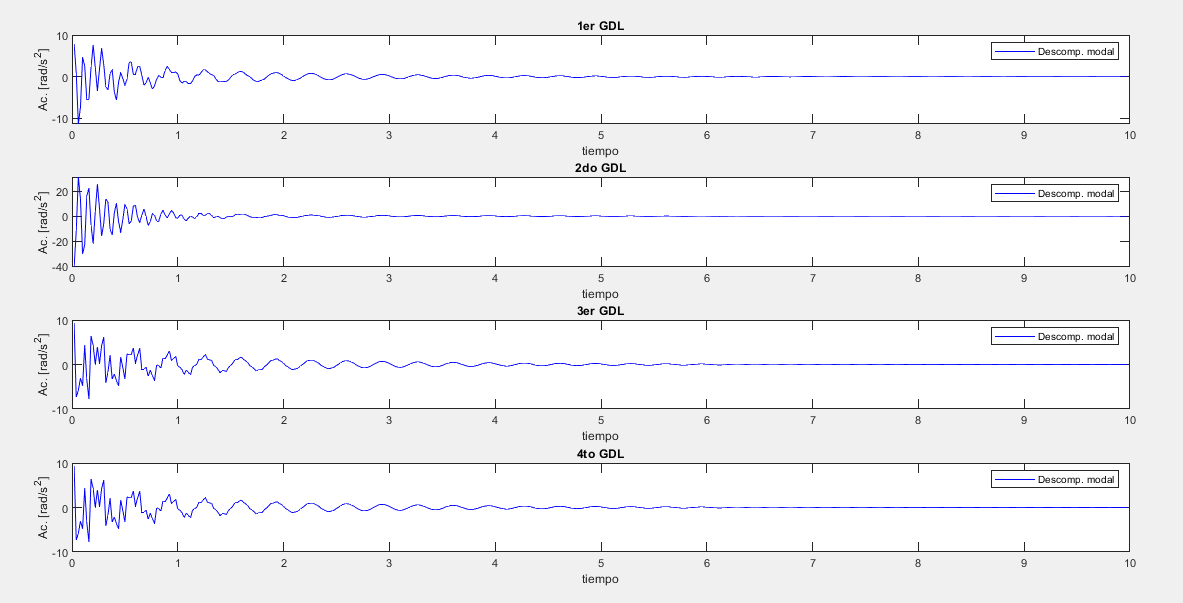
\includegraphics[width=0.90\textwidth]{Imagenes/r6.png}
    \caption{Gráfica de aceleración}
    \label{fig:etiqueta de la figura}
\end{figure}


\subsection{Para $X_0$=[0, 0, 0, 0] y $V_0$=[0, 0, 0.873, 0] y considerando que no tenemos carga adicional en el efector final ($m_4$= 310kg):}
\begin{figure}[H]
    \centering
    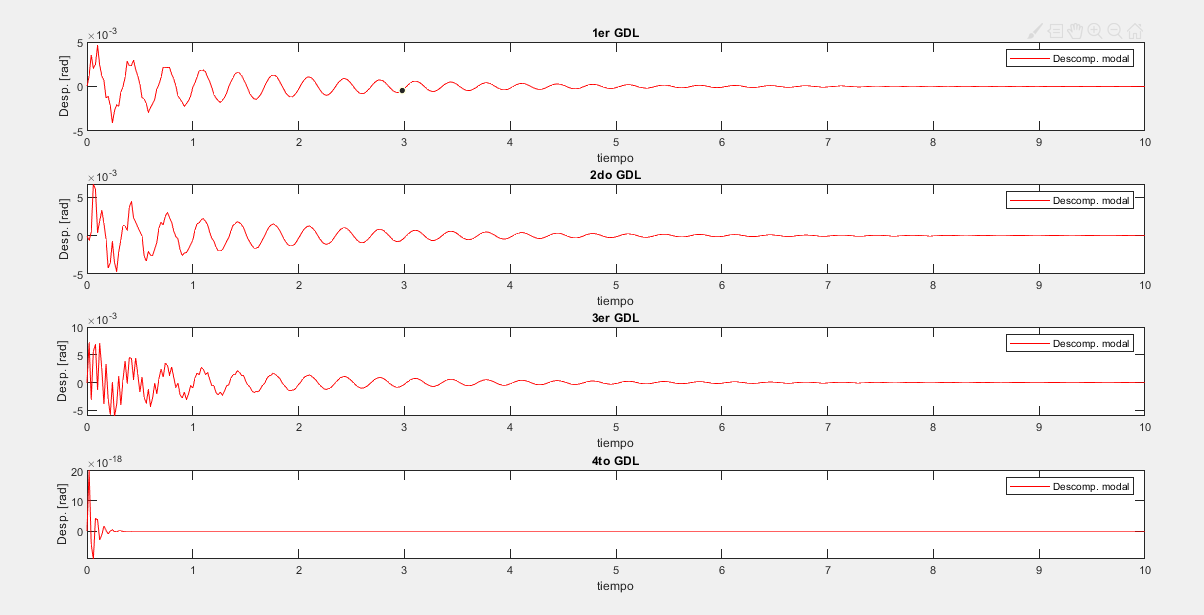
\includegraphics[width=0.90\textwidth]{Imagenes/r7.png}
    \caption{Gráfica de posición}
    \label{fig:etiqueta de la figura}
\end{figure}

\begin{figure}[H]
    \centering
    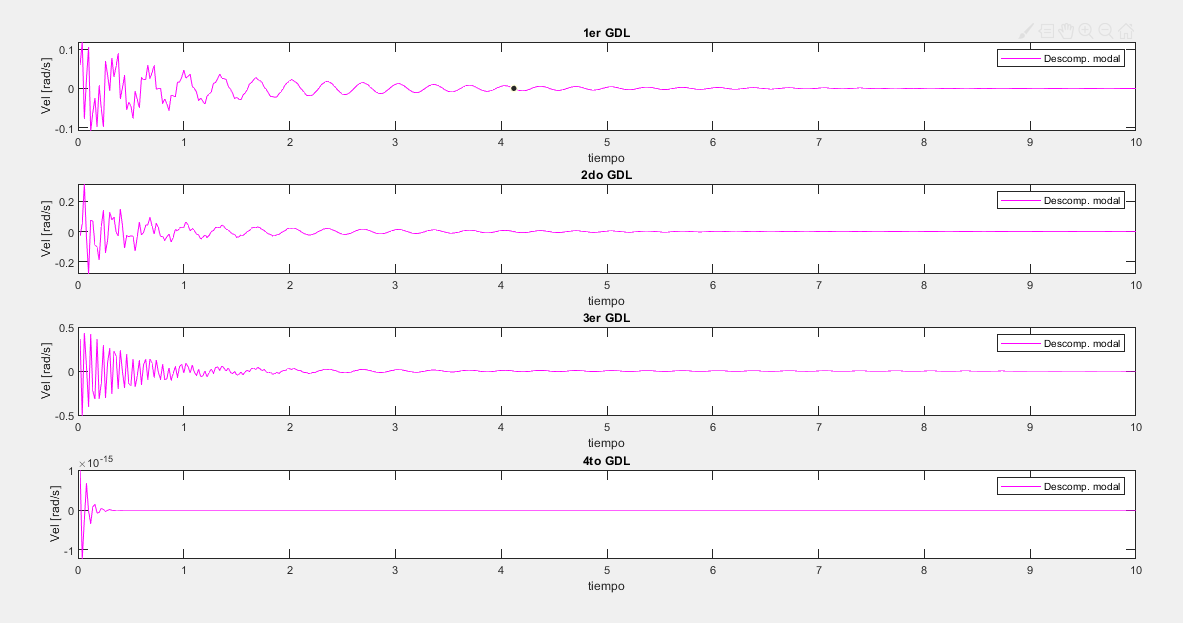
\includegraphics[width=0.90\textwidth]{Imagenes/r8.png}
    \caption{Gráfica de velocidad}
    \label{fig:etiqueta de la figura}
\end{figure}

\begin{figure}[H]
    \centering
    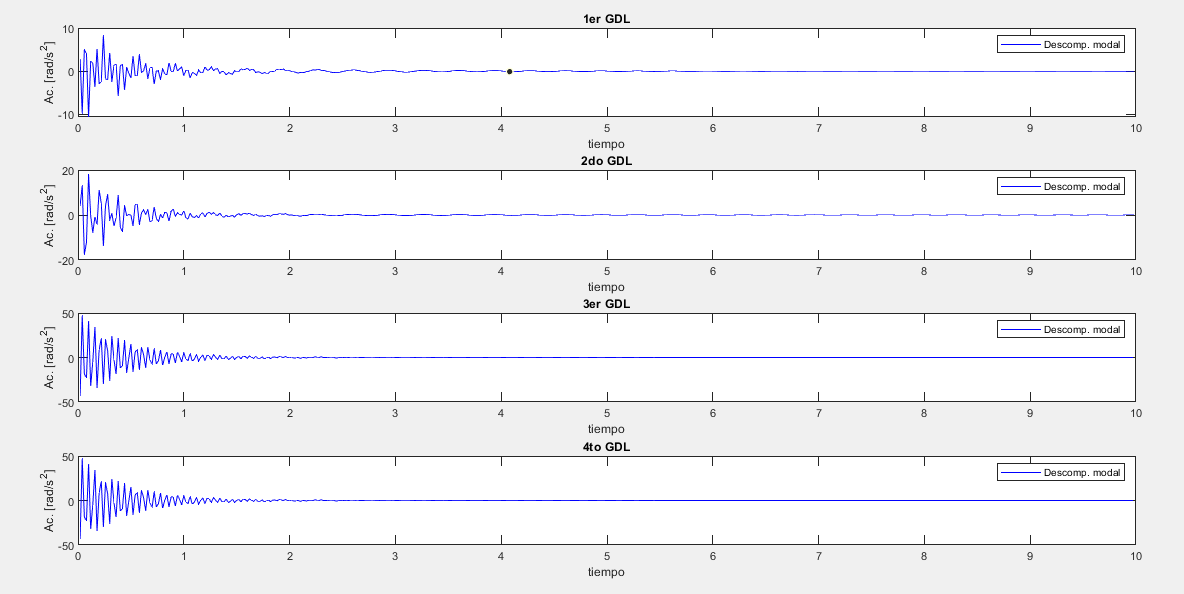
\includegraphics[width=0.90\textwidth]{Imagenes/r9.png}
    \caption{Gráfica de aceleración}
    \label{fig:etiqueta de la figura}
\end{figure}


\subsection{Para $X_0$=[0, 0, 0, 0] y $V_0$=[0, 0, 0, 1.0472] y considerando que no tenemos carga adicional en el efector final ($m_4$= 310kg):}
\begin{figure}[H]
    \centering
    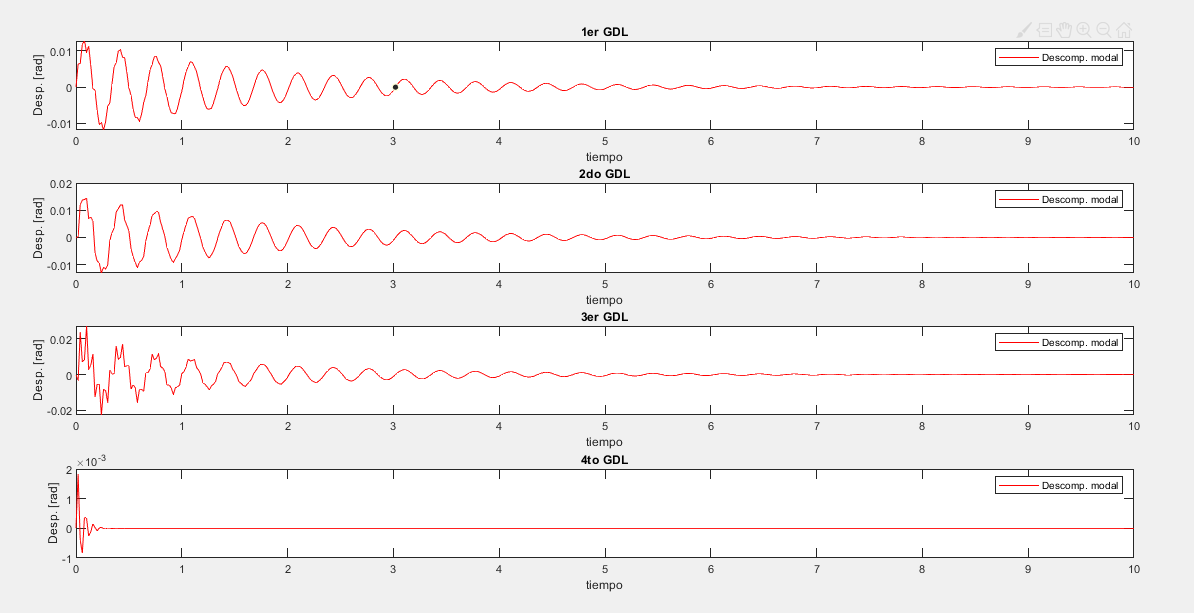
\includegraphics[width=0.90\textwidth]{Imagenes/r10.png}
    \caption{Gráfica de posición}
    \label{fig:etiqueta de la figura}
\end{figure}

\begin{figure}[H]
    \centering
    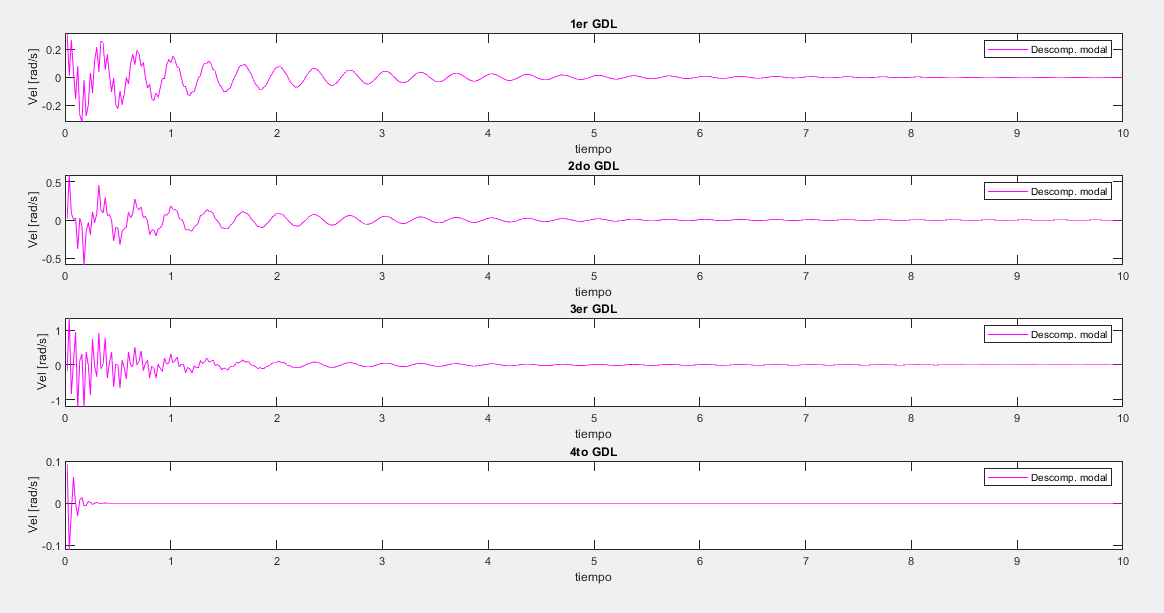
\includegraphics[width=0.90\textwidth]{Imagenes/r11.png}
    \caption{Gráfica de velocidad}
    \label{fig:etiqueta de la figura}
\end{figure}

\begin{figure}[H]
    \centering
    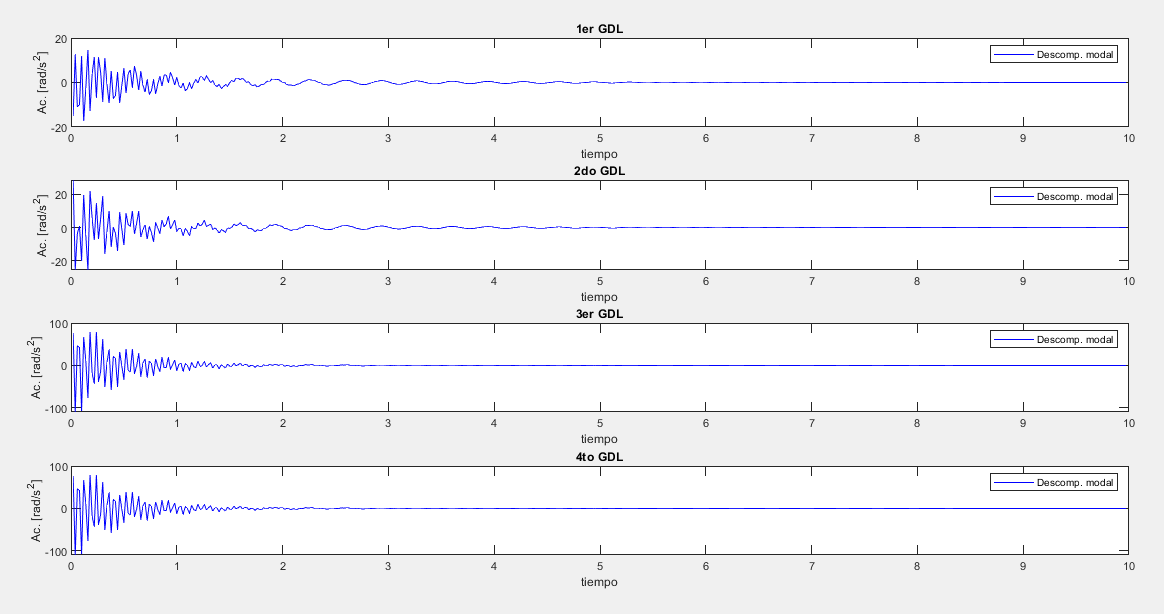
\includegraphics[width=0.90\textwidth]{Imagenes/r12.png}
    \caption{Gráfica de aceleración}
    \label{fig:etiqueta de la figura}
\end{figure}


\subsection{Para $X_0$=[0, 0, 0, 0] y $V_0$=[1.0123, 0.873, 0.873, 1.0472] y considerando que no tenemos carga adicional en el efector final ($m_4$= 310kg):}

Analizamos el caso para cuando todos los motores tienen una velocidad inicial, es decir:

\begin{figure}[H]
    \centering
    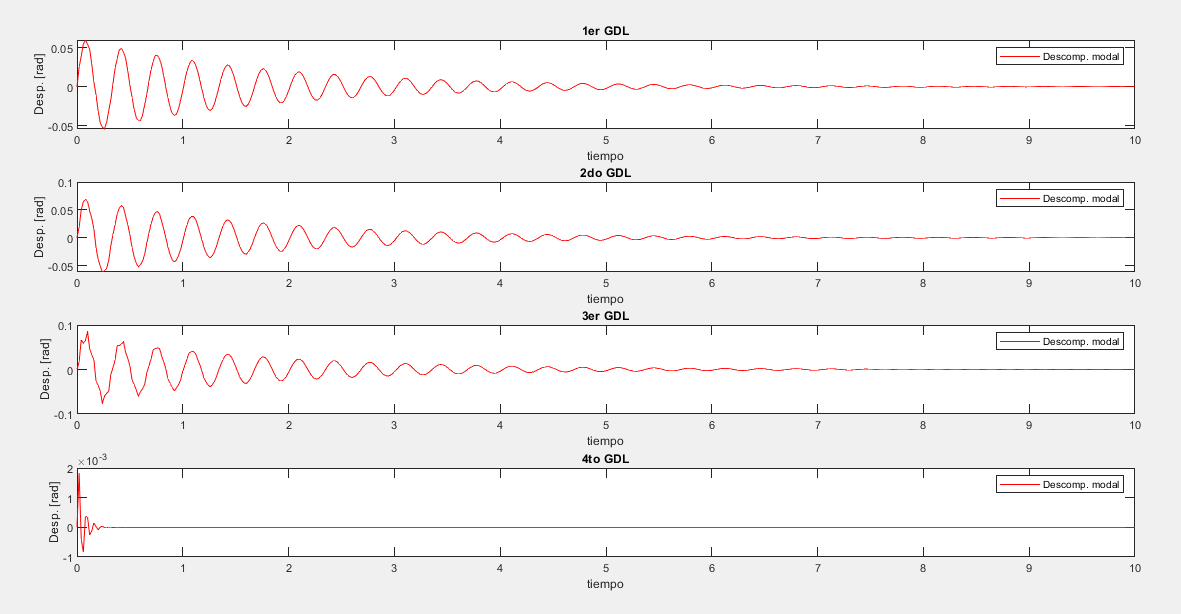
\includegraphics[width=0.90\textwidth]{Imagenes/r13.png}
    \caption{Gráfica de posición}
    \label{fig:etiqueta de la figura}
\end{figure}

\begin{figure}[H]
    \centering
    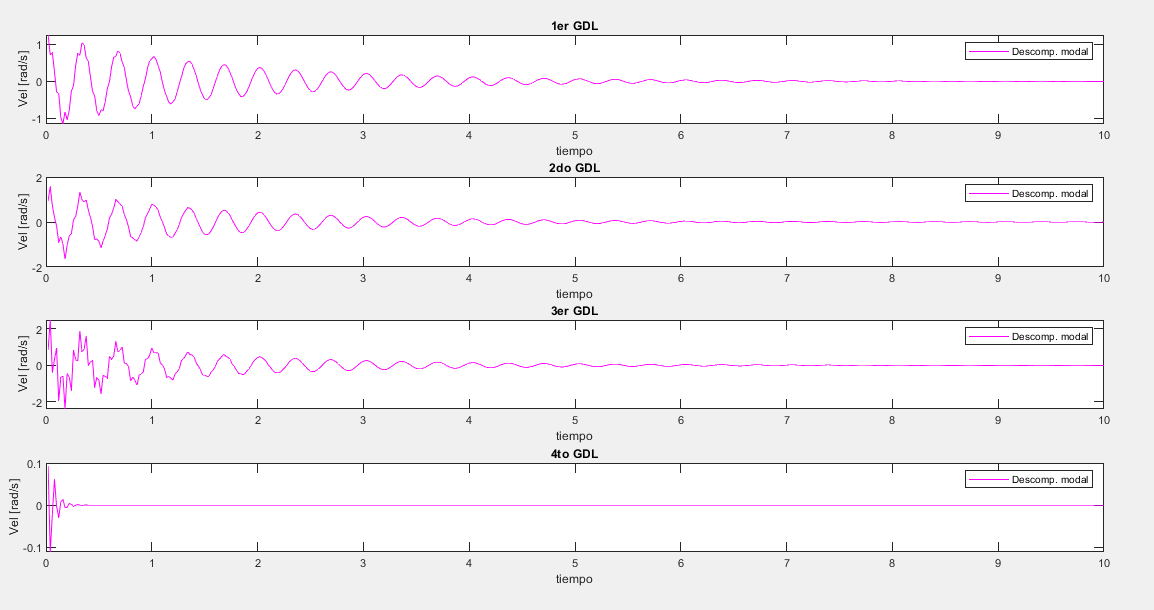
\includegraphics[width=0.90\textwidth]{Imagenes/r14.png}
    \caption{Gráfica de velocidad}
    \label{fig:etiqueta de la figura}
\end{figure}

\begin{figure}[H]
    \centering
    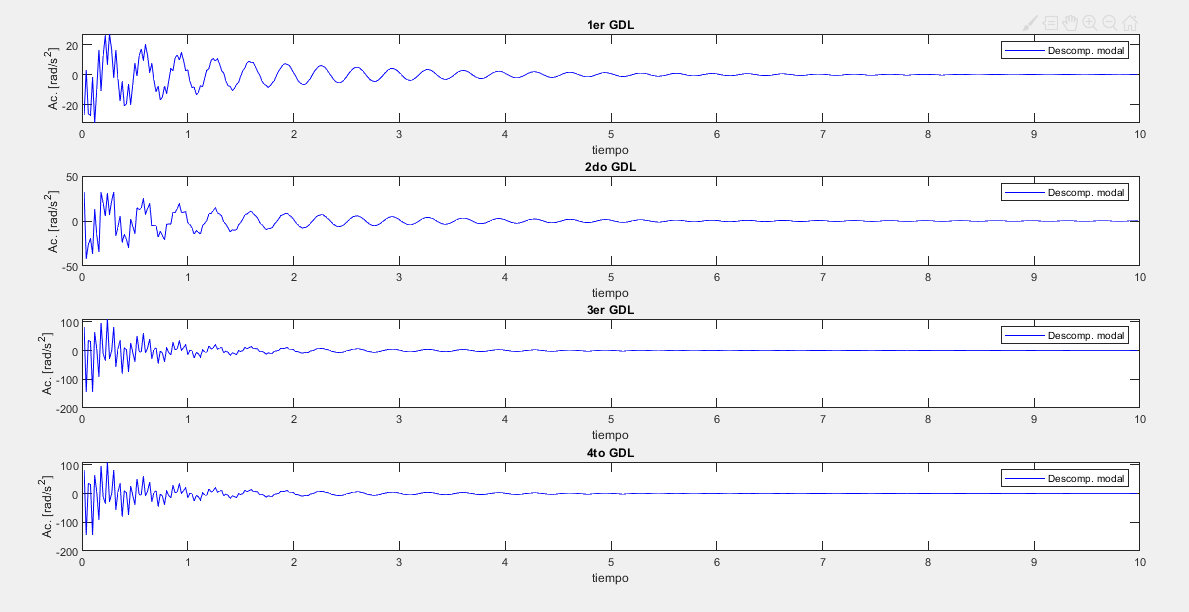
\includegraphics[width=0.90\textwidth]{Imagenes/r15.png}
    \caption{Gráfica de aceleración}
    \label{fig:etiqueta de la figura}
\end{figure}


\subsection{Para $X_0$=[0, 0, 0, 0] y $V_0$=[1.0123, 0, 0, 0] y considerando que se tiene carga adicional en el efector final ($m_4$= 810 kg):}

Ahora consideraremos una carga que se sostiene en el efector final de 500kg, por lo cual $m_4$ aumentará de 310kg a 810 kg.


\begin{figure}[H]
    \centering
    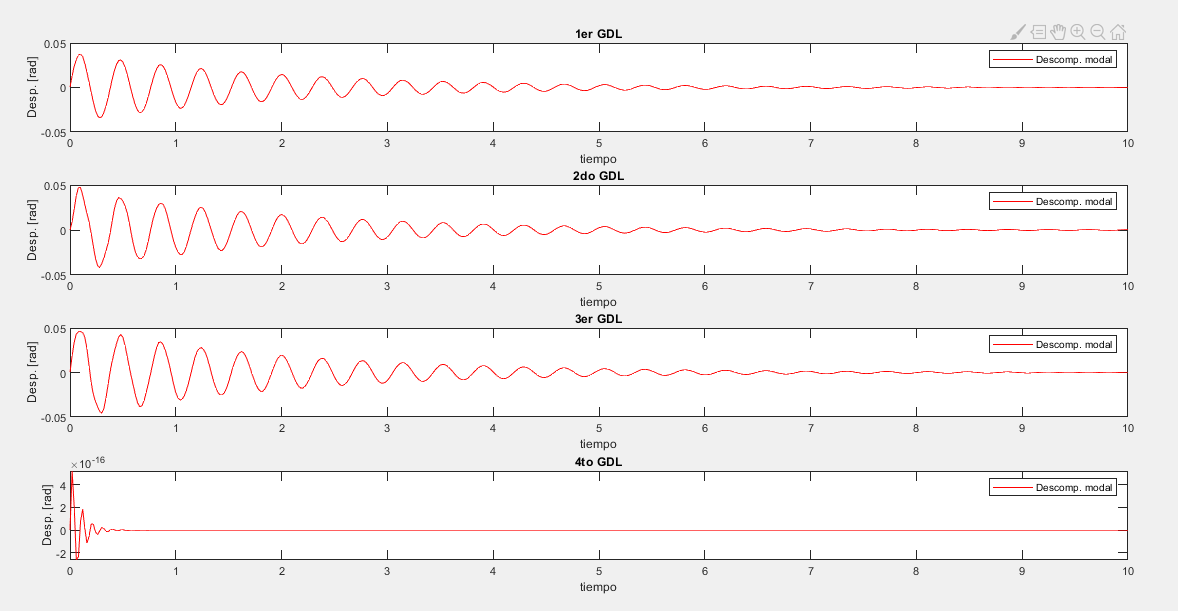
\includegraphics[width=0.90\textwidth]{Imagenes/r16.png}
    \caption{Gráfica de posición}
    \label{fig:etiqueta de la figura}
\end{figure}

\begin{figure}[H]
    \centering
    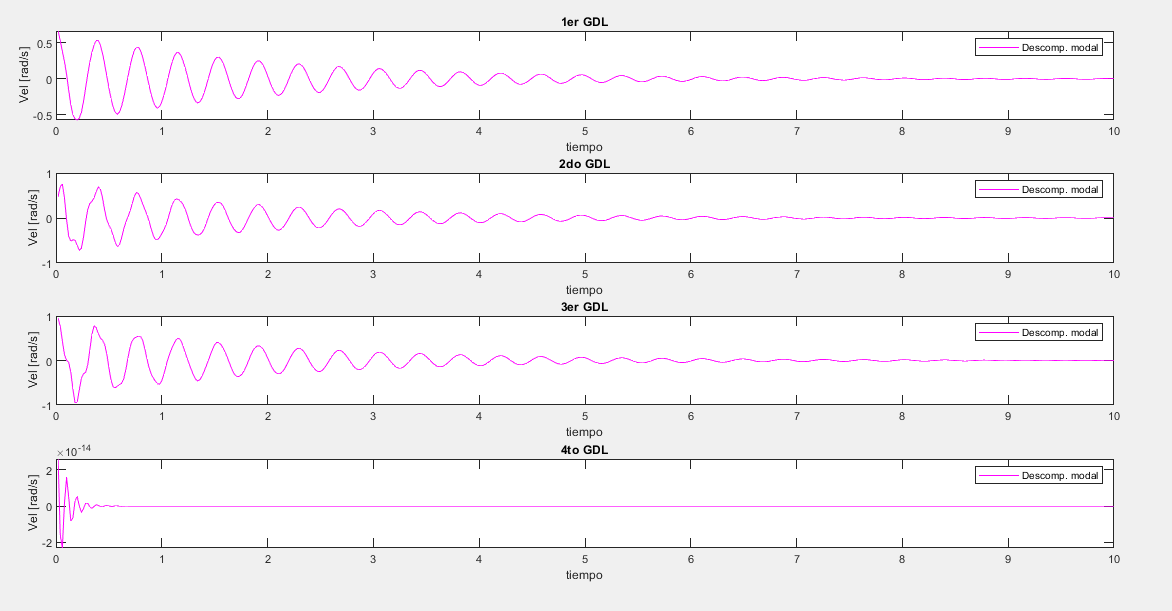
\includegraphics[width=0.90\textwidth]{Imagenes/r17.png}
    \caption{Gráfica de velocidad}
    \label{fig:etiqueta de la figura}
\end{figure}

\begin{figure}[H]
    \centering
    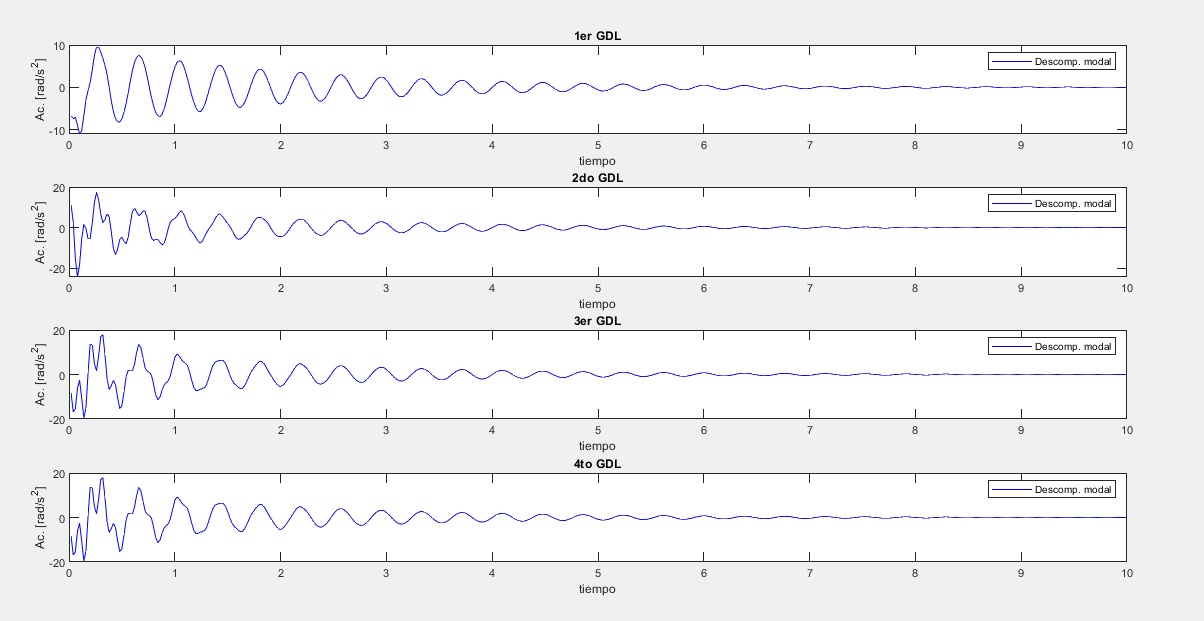
\includegraphics[width=0.90\textwidth]{Imagenes/r18.png}
    \caption{Gráfica de aceleración}
    \label{fig:etiqueta de la figura}
\end{figure}


\subsection{Para $X_0$=[0, 0, 0, 0] y $V_0$=[0, 0.873, 0, 0] y considerando que se tiene carga adicional en el efector final ($m_4$= 810 kg):}
\begin{figure}[H]
    \centering
    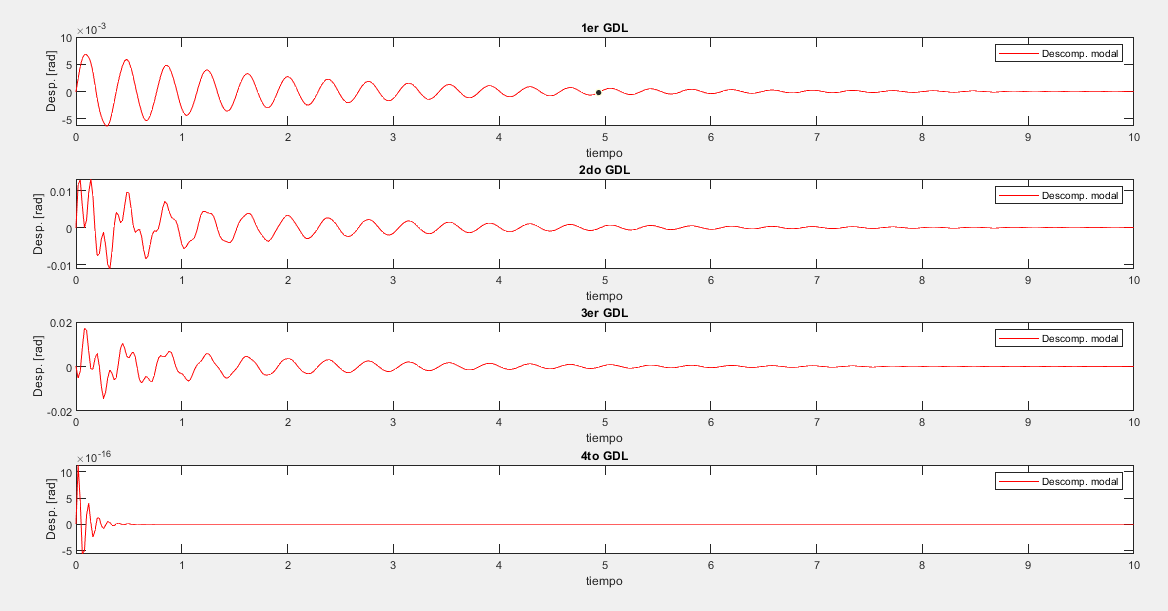
\includegraphics[width=0.90\textwidth]{Imagenes/r19.png}
    \caption{Gráfica de posición}
    \label{fig:etiqueta de la figura}
\end{figure}

\begin{figure}[H]
    \centering
    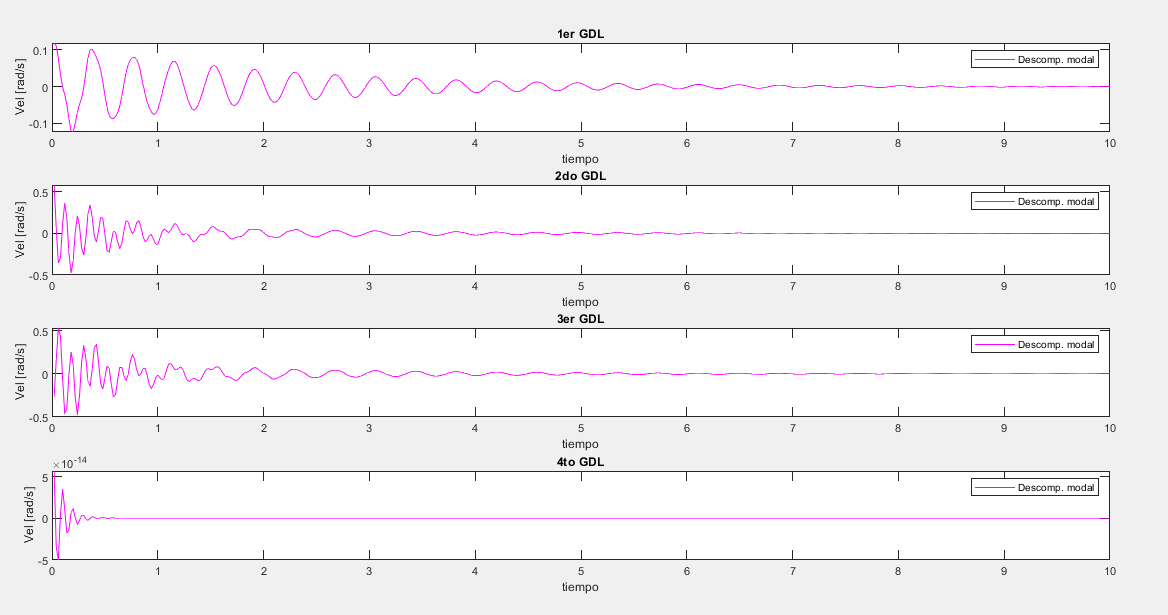
\includegraphics[width=0.90\textwidth]{Imagenes/r20.png}
    \caption{Gráfica de velocidad}
    \label{fig:etiqueta de la figura}
\end{figure}

\begin{figure}[H]
    \centering
    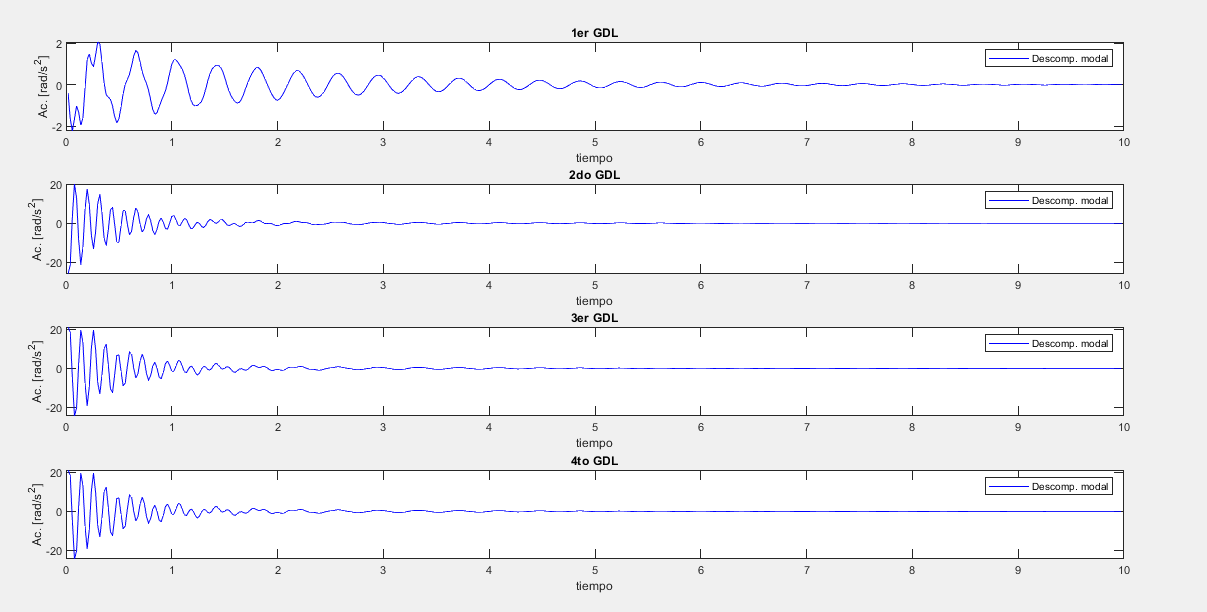
\includegraphics[width=0.90\textwidth]{Imagenes/r21.png}
    \caption{Gráfica de aceleración}
    \label{fig:etiqueta de la figura}
\end{figure}


\subsection{Para $X_0$=[0, 0, 0, 0] y $V_0$=[0, 0, 0.873, 0] y considerando que se tiene carga adicional en el efector final ($m_4$= 810 kg):}
\begin{figure}[H]
    \centering
    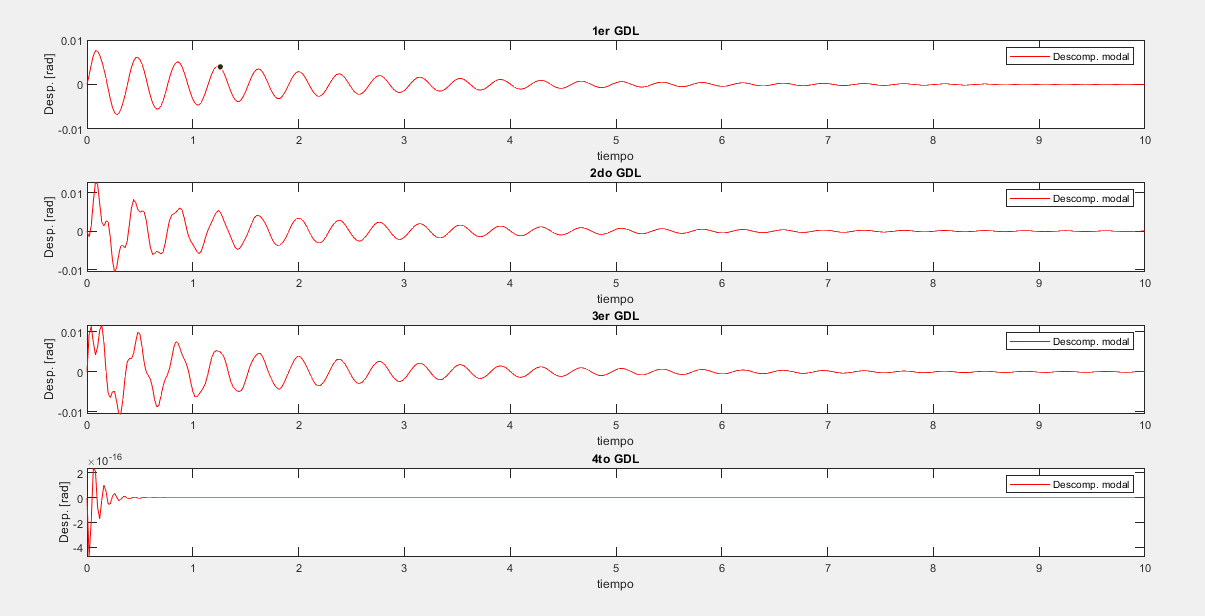
\includegraphics[width=0.90\textwidth]{Imagenes/r22.png}
    \caption{Gráfica de posición}
    \label{fig:etiqueta de la figura}
\end{figure}

\begin{figure}[H]
    \centering
    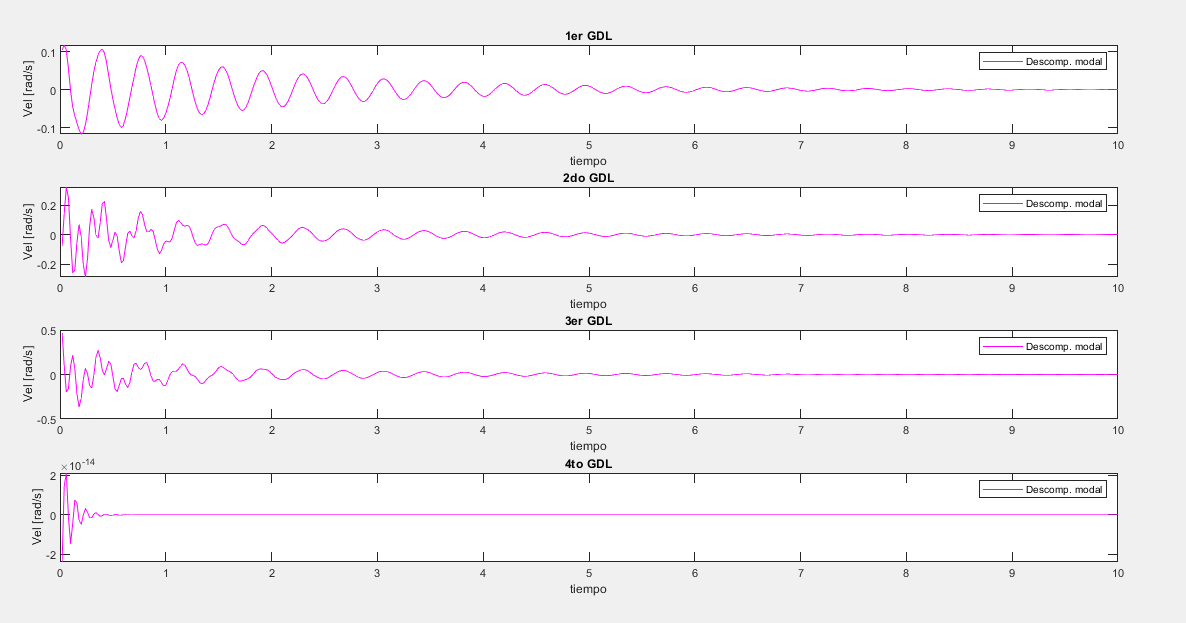
\includegraphics[width=0.90\textwidth]{Imagenes/r23.png}
    \caption{Gráfica de velocidad}
    \label{fig:etiqueta de la figura}
\end{figure}

\begin{figure}[H]
    \centering
    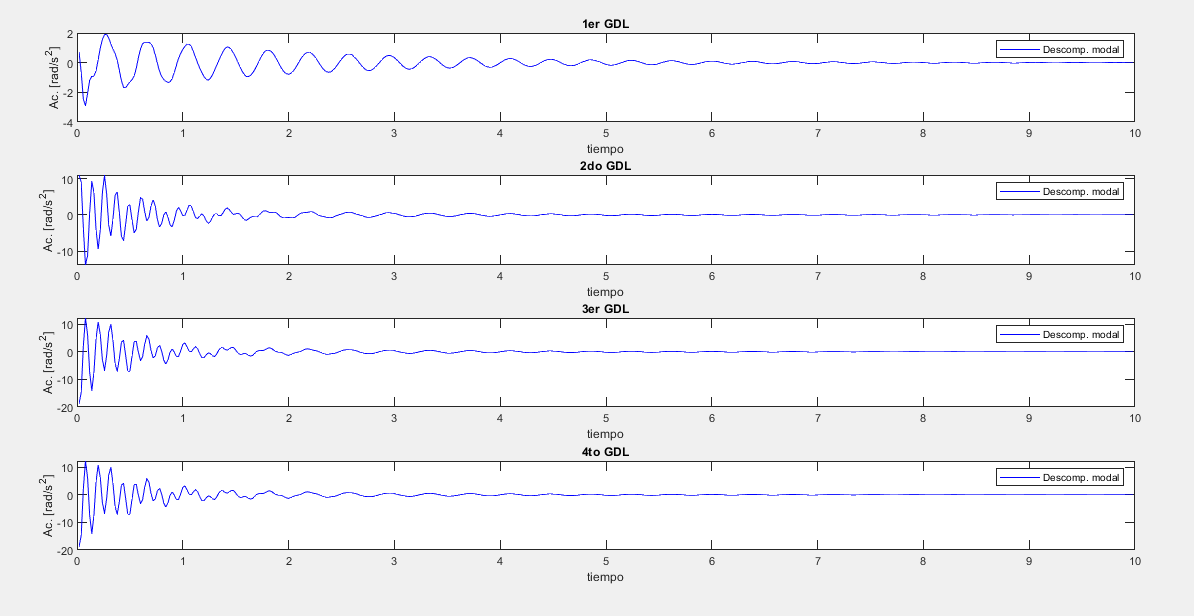
\includegraphics[width=0.90\textwidth]{Imagenes/r24.png}
    \caption{Gráfica de aceleración}
    \label{fig:etiqueta de la figura}
\end{figure}


\subsection{Para $X_0$=[0, 0, 0, 0] y $V_0$=[0, 0, 0, 1.0472] y considerando que se tiene carga adicional en el efector final ($m_4$= 810 kg):}
\begin{figure}[H]
    \centering
    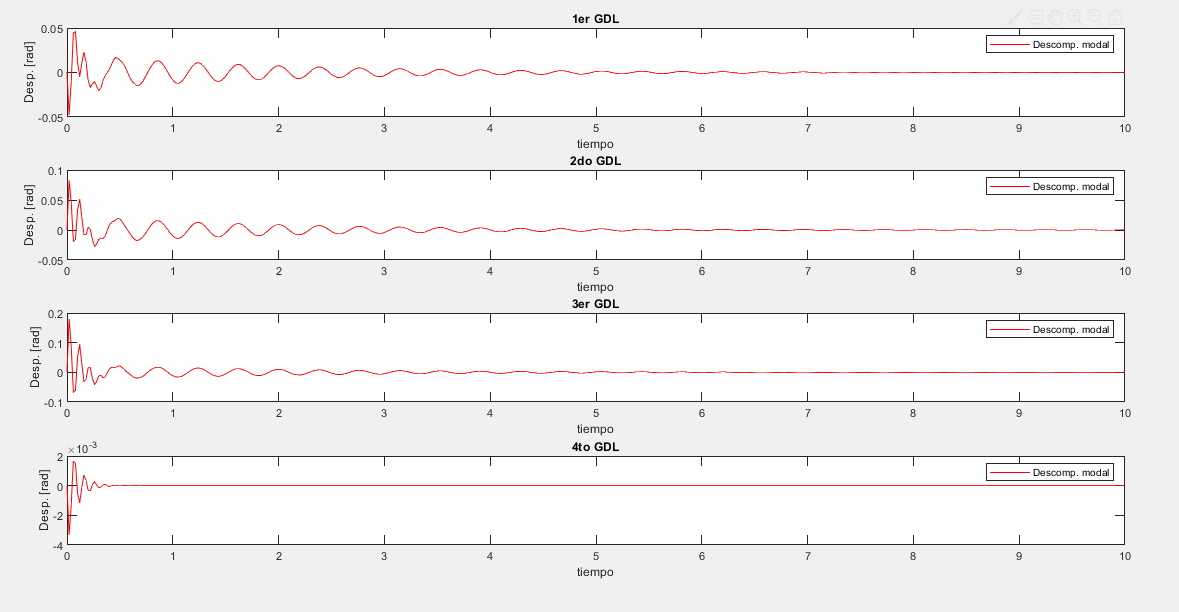
\includegraphics[width=0.90\textwidth]{Imagenes/r25.png}
    \caption{Gráfica de posición}
    \label{fig:etiqueta de la figura}
\end{figure}

\begin{figure}[H]
    \centering
    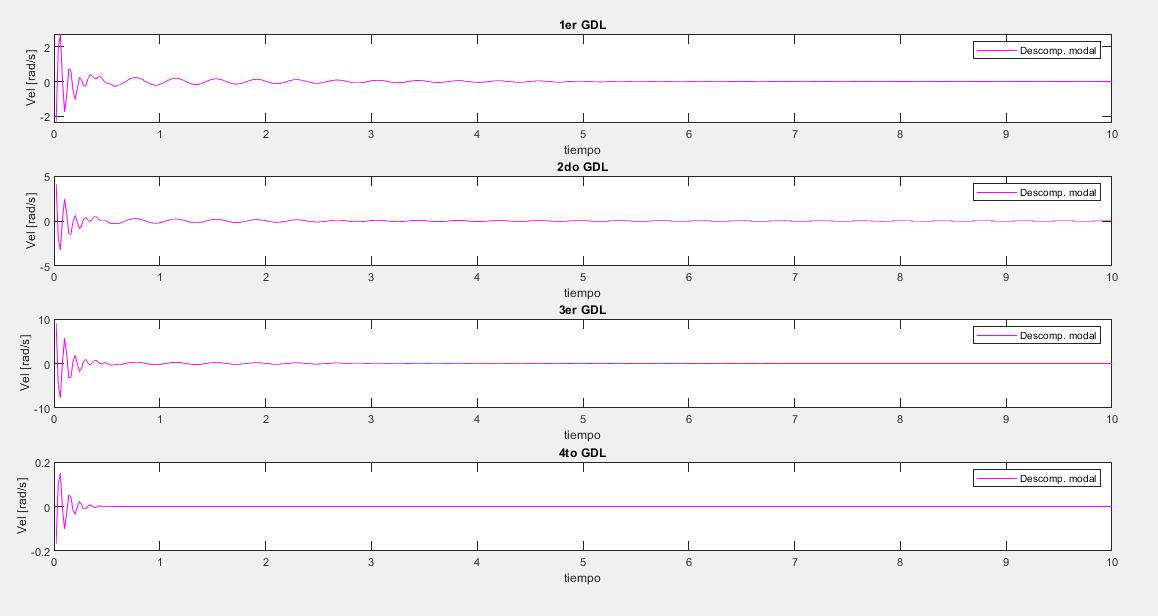
\includegraphics[width=0.90\textwidth]{Imagenes/r26.png}
    \caption{Gráfica de velocidad}
    \label{fig:etiqueta de la figura}
\end{figure}

\begin{figure}[H]
    \centering
    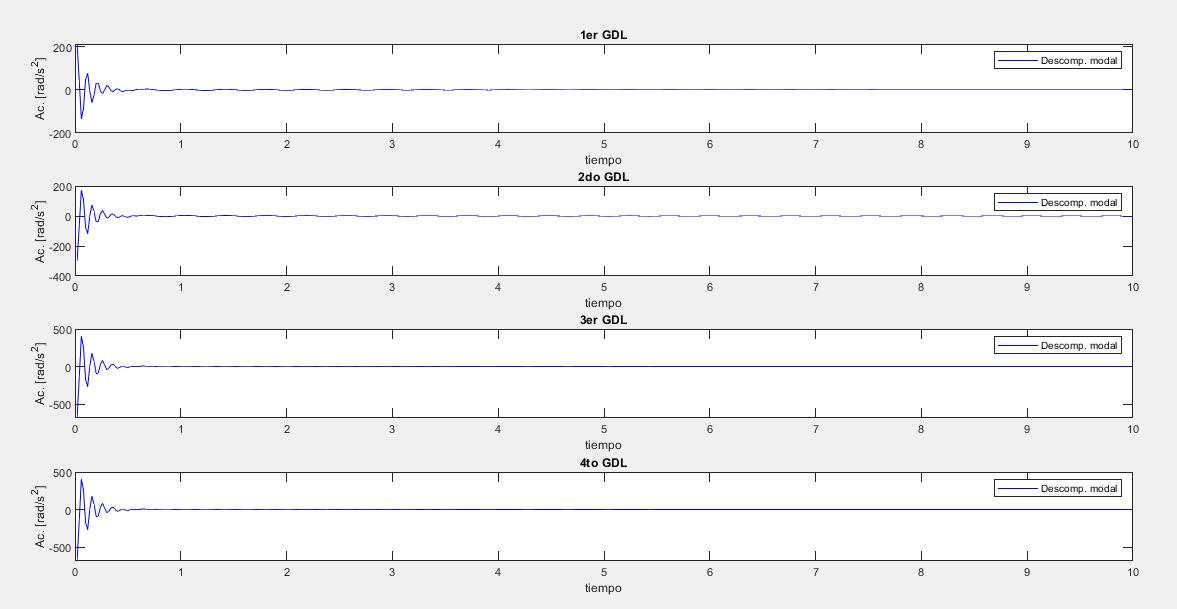
\includegraphics[width=0.90\textwidth]{Imagenes/r27.png}
    \caption{Gráfica de aceleración}
    \label{fig:etiqueta de la figura}
\end{figure}


\subsection{ Para $X_0$=[0, 0, 0, 0] y $V_0$=[1.0123, 0.873, 0.873, 1.0472] y considerando que se tiene carga adicional en el efector final ($m_4$= 810 kg):}
\begin{figure}[H]
    \centering
    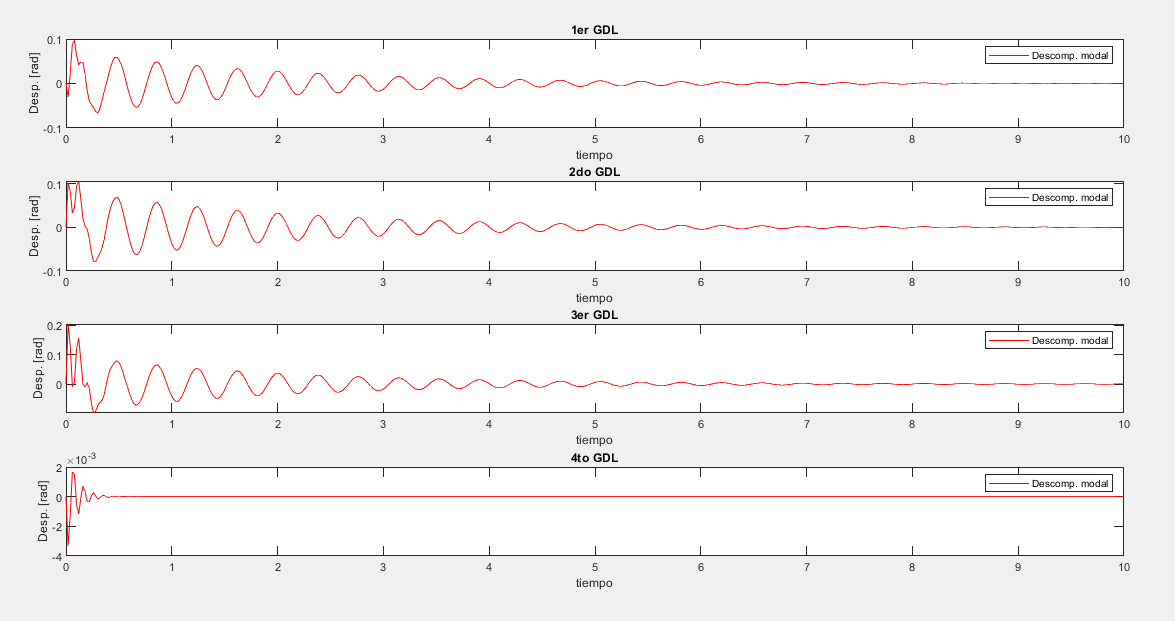
\includegraphics[width=0.90\textwidth]{Imagenes/r28.png}
    \caption{Gráfica de posición}
    \label{fig:etiqueta de la figura}
\end{figure}

\begin{figure}[H]
    \centering
    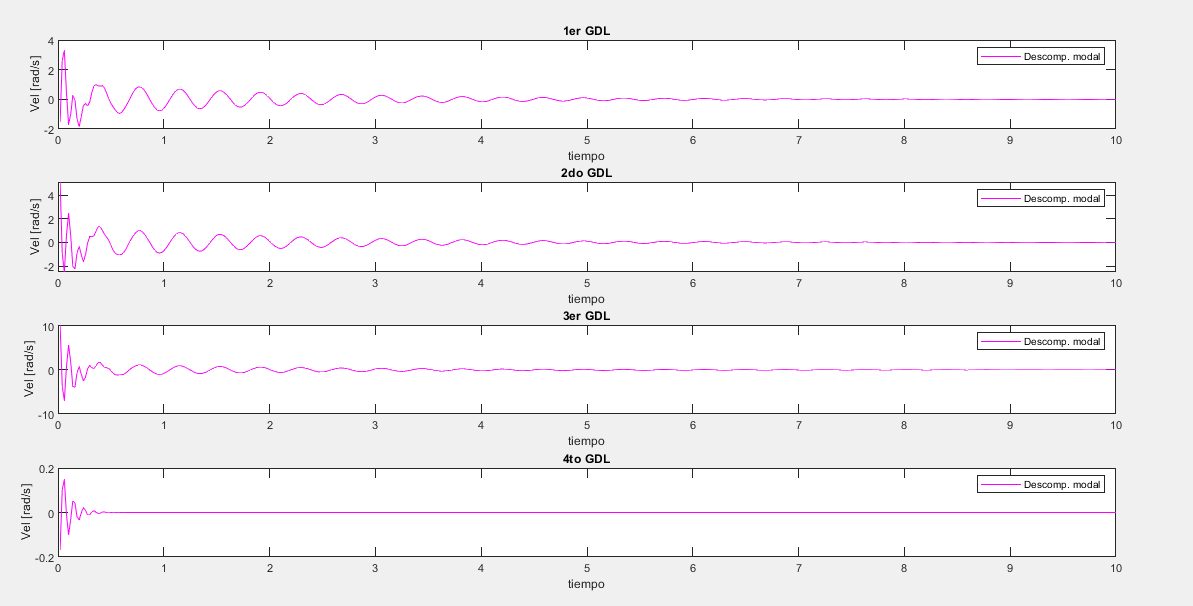
\includegraphics[width=0.90\textwidth]{Imagenes/r29.png}
    \caption{Gráfica de velocidad}
    \label{fig:etiqueta de la figura}
\end{figure}

\begin{figure}[H]
    \centering
    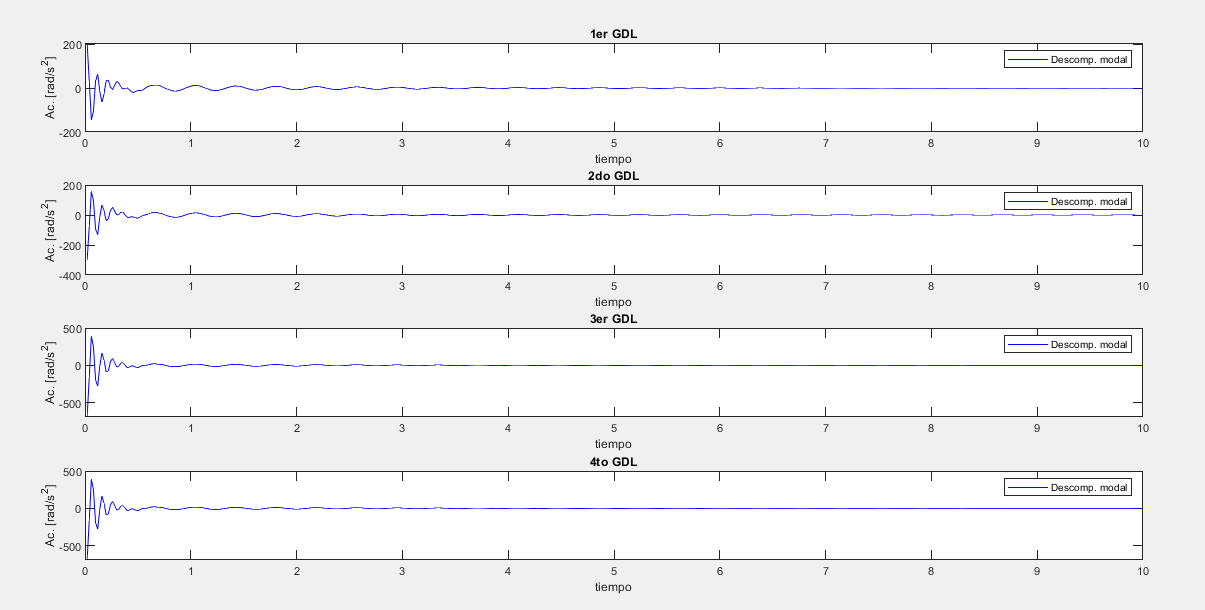
\includegraphics[width=0.90\textwidth]{Imagenes/r30.png}
    \caption{Gráfica de aceleración}
    \label{fig:etiqueta de la figura}
\end{figure}

%%%%%%%%%%%%%%%%%%%%%%%%%%%%%%%%%%%%%%%%
\section{Análisis de Datos obtenidos}
%%%%%%%%%%%%%%%%%%%%%%%%%%%%%%%%%%%%%%%%

Para realizar una comparación, analizaremos el caso en el que se considera una velocidad inicial para el 1° gdl y otro para todos los grados de libertad con y sin carga.

\begin{figure}[H]
    \centering
    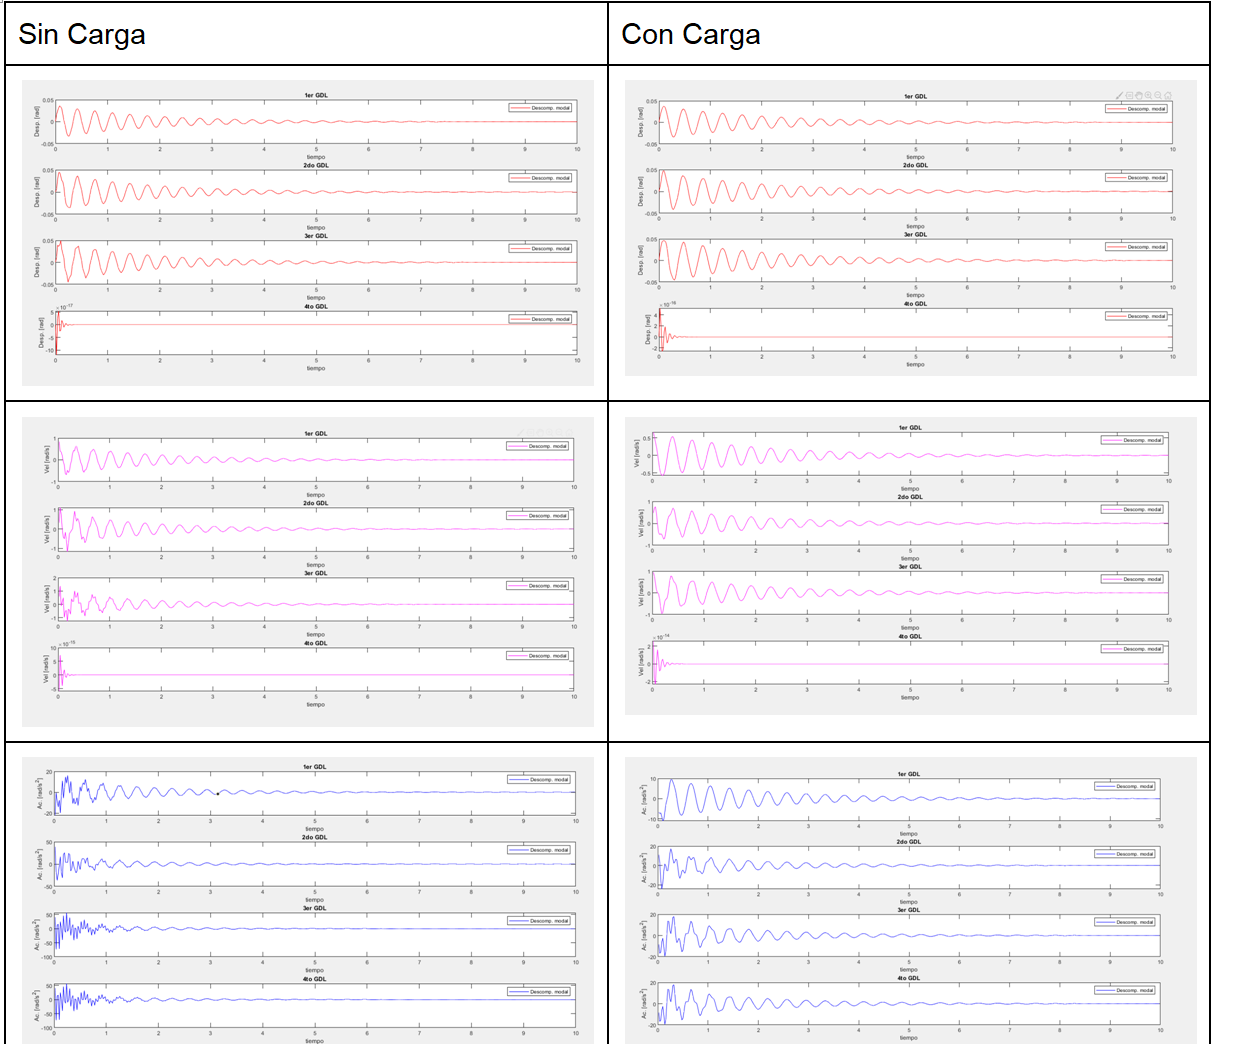
\includegraphics[width=0.90\textwidth]{Imagenes/V01GDL.png}
    \caption{Para V0=[1.0123, 0, 0, 0]}
    \label{fig:etiqueta de la figura}
\end{figure}

\begin{figure}[H]
    \centering
    \includegraphics[width=0.90\textwidth]{Imagenes/V0todos.png}
    \caption{Para V0=[1.0123, 0.873, 0.873, 1.0472]}
    \label{fig:etiqueta de la figura}
\end{figure}

Analizando los primeros 3 gdl que son más representativos en nuestro sistema, si damos una condición inicial de Velocidad en todos los gdl (el peor de los casos) con o sin carga:

\subsection{Para $X_0$=[0, 0, 0, 0] y $V_0$=[1.0123, 0, 0, 0]}

\begin{figure}[H]
    \centering
    \includegraphics[width=1\textwidth]{Imagenes/t1.png}
    \caption{Tabla(1). Parámetros Máximos y Mínimos ante condición inicial de velocidad en 1° GDL sin carga adicional
}
    \label{fig:etiqueta de la figura}
\end{figure}

\begin{figure}[H]
    \centering
    \includegraphics[width=1\textwidth]{Imagenes/t2.png}
    \caption{Tabla(2). Parámetros Máximos y Mínimos ante condición inicial de velocidad en 1° GDL con carga adicional}
    \label{fig:etiqueta de la figura}
\end{figure}

En el caso que el primer servo se moviera a máxima velocidad, se puede observar que el 1° gdl, con una amplitud máxima absoluta en desplazamiento sin carga de 0.067 rad(3.83°) y con carga de 0.071 rad(4.068°). Comparando las gráficas con el siguiente paper: Vibration damping control of robot arm intended for service application in human environment.

Logramos obtener resultados similares ante los resultados experimentales en la magnitud de la oscilación en desplazamiento del 1° GDL. Por lo cual podemos asegurar que el sistema resiste cambios en la velocidad angular y provee un comportamiento dinámico fluido.

El sistema rechaza perturbaciones de tal forma que podemos afirmar que el sistema ya no vibra luego de 4  segundos

El gdl más afectado es el 3° gdl,con una amplitud máxima absoluta en desplazamiento sin carga de 0.09 rad(5.15°) y con carga de 0.09 rad(5.15°)


\begin{figure}[H]
    \centering
    \includegraphics[width=1\textwidth]{Imagenes/t3.png}
    \caption{Tabla(3). Parámetros Máximos y Mínimos ante condición inicial de velocidad en cada GDL sin carga adicional}
    \label{fig:etiqueta de la figura}
\end{figure}

\begin{figure}[H]
    \centering
    \includegraphics[width=1\textwidth]{Imagenes/t4.png}
    \caption{Tabla(4). Parámetros Máximos y Mínimos ante condición inicial de velocidad en cada GDL con carga adicional}
    \label{fig:etiqueta de la figura}
\end{figure}

En el caso que todos los servos se movieran al mismo tiempo a máxima velocidad, podemos observar que el gdl más afectado es el 3° gdl, con una amplitud máxima absoluta en desplazamiento sin carga de 0.16 rad(9.16°) y con carga de 0.298 rad (17.07°).


%%%%%%%%%%%%%%%%%%%%%%%%%%%%%%%%%%%%%%%%
\section{Conclusiones}
%%%%%%%%%%%%%%%%%%%%%%%%%%%%%%%%%%%%%%%%

Respecto a la Estructura y comportamiento Robot KUKA:
Analizando la tabla(1), y observando el desplazamiento sufrido por el 1° gdl al momento de darle una condición inicial de velocidad a este, podemos observar que el valor máximo de desplazamiento en grados es de cerca 1.8°, el cual se atenúa totalmente luego de 4 segundos.Al compararlo con otros estudios y papers podemos asegurar que es un valor aceptable y describe un buen comportamiento del brazo robótico.

Analizando la tabla(4), observamos que este es el caso más exigido y en sí poco probable, ya que en la realidad no es común que se desplacen más de 2 articulaciones al mismo tiempo a máxima velocidad, y además sosteniendo una carga adicional m4=500kg. Podemos observar que el valor máximo de desplazamiento en grados es de cerca 9.5°, el cual se atenúa totalmente luego de 5 segundos. También se puede observar que al momento de sostener la carga adicional, las aceleraciones angulares aumentan en gran medida.


%%%%%%%%%%%%%%%%%%%%%%%%%%%%%%%%%%%%%%%%
\section{Bibliografía y citas}
%%%%%%%%%%%%%%%%%%%%%%%%%%%%%%%%%%%%%%%%

La bibliografía debe incluirse mediante un archivo \texttt{.bib} con el mismo nombre que el archivo principal y utilizando el paquete \texttt{biblatex} (ya incluido en la clase). Únicamente deben incluirse referencias citadas en el artículo.

El estilo bibliográfico a usar es APA séptima edición, algunos ejemplos e información se pueden encontrar en: \url{https://apastyle.apa.org/style-grammar-guidelines/references/examples}. Y una versión traducida en: \url{https://normasapa.pro/}.

Para las citas puede utilizar los siguientes comandos según sea adecuado:
\begin{itemize}
\item 
    Cita completa entre paréntesis \verb"\parencite{ }": \parencite{Bib06}
\item
    Cita completa sin paréntesis \verb"\textcite{ }": \textcite{Bib06}
\item 
    Cita completa entre paréntesis \verb"\cite{ }": \cite{Bib06}
\item
    Cita de autor \verb"\citeauthor{ }": \citeauthor{Bib06}
\item
    Cita de año \verb"\citeyear{ }": \citeyear{Bib06}
\item 
    Cita con opciones extras \verb"\parencite[ ][ ]{ }": \parencite[ver][pág. 66]{Bib06}
\end{itemize}
Información adicional sobre el paquete \texttt{biblatex} puede encontrarse en: \url{http://tug.ctan.org/info/biblatex-cheatsheet/biblatex-cheatsheet.pdf}

Finalmente, se presentan ejemplos de referencias que se pueden utilizar:
\begin{itemize}
    \item Artículos de revista: \cite{Bib01}
    \item Libros: \cite{Bib02}
    \item Libros: \cite{Bib06}
    \item Tesis: \cite{Bib03}
    \item Sitios web: \cite{Bib04}
    \item Videos: \cite{Bib05}
\end{itemize}

%%%%%%%%%%%%%%%%%%%%%%%%%%%%%%%%%%%%%%%%
%% Referencias
%%%%%%%%%%%%%%%%%%%%%%%%%%%%%%%%%%%%%%%%
\printbibliography



\end{document}